
\subsection{シミュレーション実験の目的}
直進動作のシミュレーション実験によって,脚軌道生成の失敗を防ぐためには,最小半径を140mmとすることが有効であるとわかった.
しかし,最小半径を140mmに設定すると,近似された脚の可動範囲が小さくなる.
そのため,先行研究の手法で歩行することができた地形であっても,歩行できなくなる可能性がある.
直進動作時については,歩行することができることを確認できたため,
本章では,旋回動作を行う際に,最小半径を140mmとした場合に,歩行できるかを検証することを目的とする.

先行研究では旋回動作は2次元空間でのみ実装されていたが,新たに3次元空間での旋回動作を実装したため,
先行研究で確認された地形を含めた3次元空間での旋回動作をシミュレーションで検証する.

\subsection{シミュレーション実験の条件}
シミュレーションを行うソフトウェア,シミュレーションを行う計算環境,
モデルとするロボットは直進動作のシミュレーション実験と同様であるため説明を省略する.
歩行条件についても直進動作のシミュレーション実験と同様とするが,
最小半径を140mmとし,動作は旋回動作とする.また,旋回は超信地旋回的に行う.

\subsubsection{歩行する地形}
先行研究でシミュレーションが行われた地形は,
平地(\figref{fig:ch5_simu_terrain_turn}(a)),
亀裂のある地形(\figref{fig:ch5_simu_terrain_turn}(b)),
溝のある地形(\figref{fig:ch5_simu_terrain_turn}(c))であるため,
これらの3つの地形でシミュレーションを行うこととした.
また,3次元空間での旋回動作を行うために,
これらの地形の中央に100mm,110mm,120mm,130mmの段差を設けた地形もシミュレーションに用いた.
さらに,これらの地形の全体を5度,10度,15度傾斜させた地形もシミュレーションに用いた.
\figref{fig:ch5_simu_terrain_turn2}は左図が平面地形に130mmの段差を設けた地形であり,
右図は平面地形を15度傾斜させた地形である.
段差を100mmから130mmとした理由は,波東らの研究によって,
胴体姿勢を変更しない場合には上ることができる段差の高さの最大値が,130mm程度であることがわかったためである.
傾斜を5度から15度とした理由も同様である.

\newpage

\begin{figure}[htbp]
  \begin{tabular}{cc}
    \begin{minipage}[t]{0.45\hsize}
      \begin{center}
      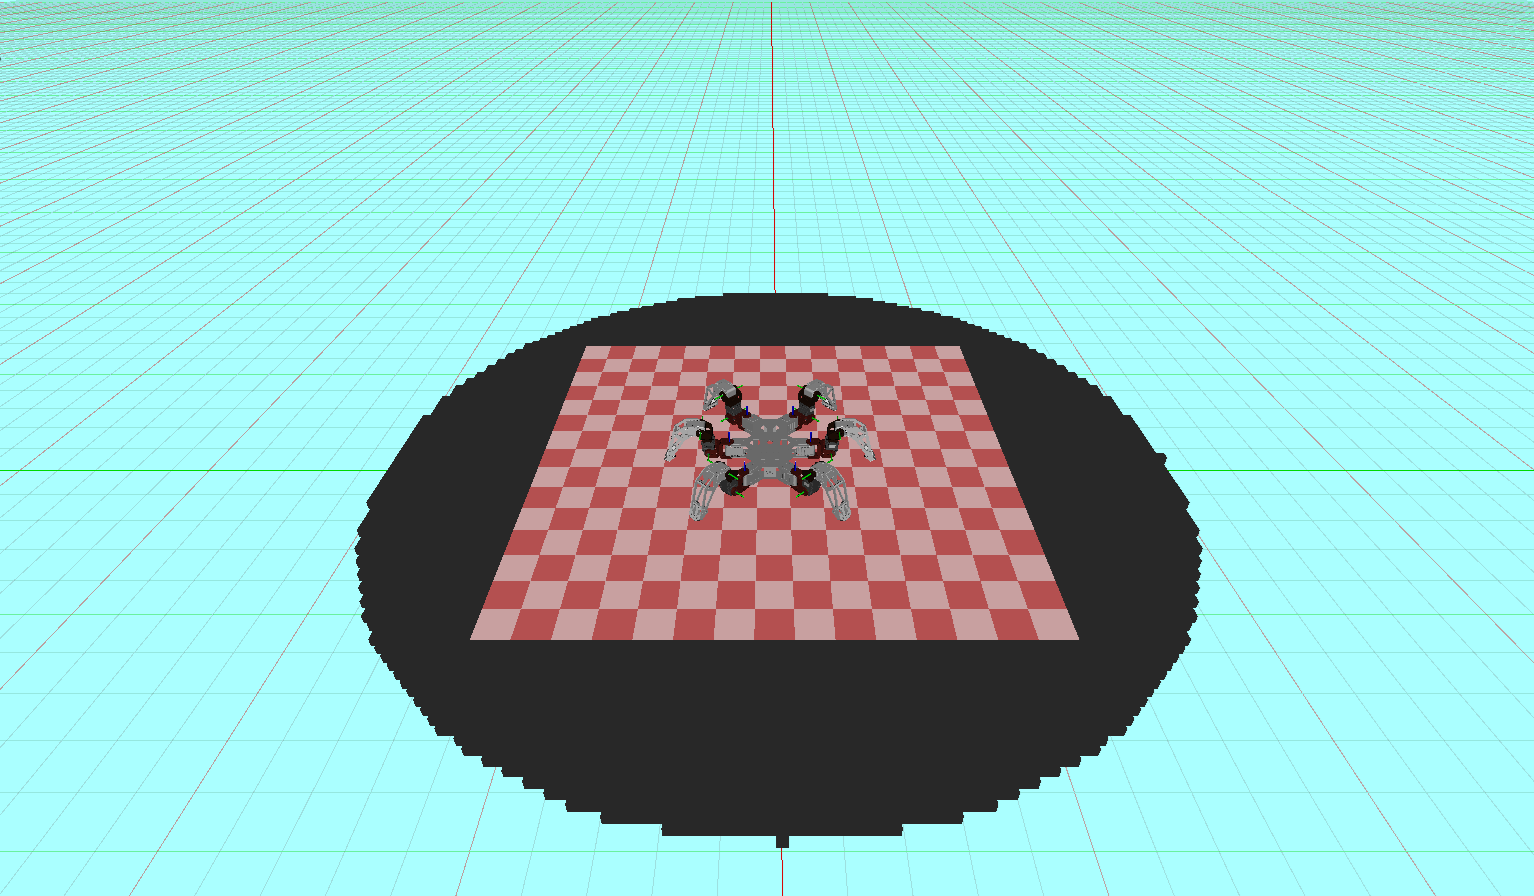
\includegraphics[width=1.0\linewidth,trim={30 30 30 30}, clip]{figure/chapter4/circle_flat.png}
      \text{(a) flat terrain}
      \end{center}
    \end{minipage} 
    &
    \begin{minipage}[t]{0.45\hsize}
      \begin{center}
      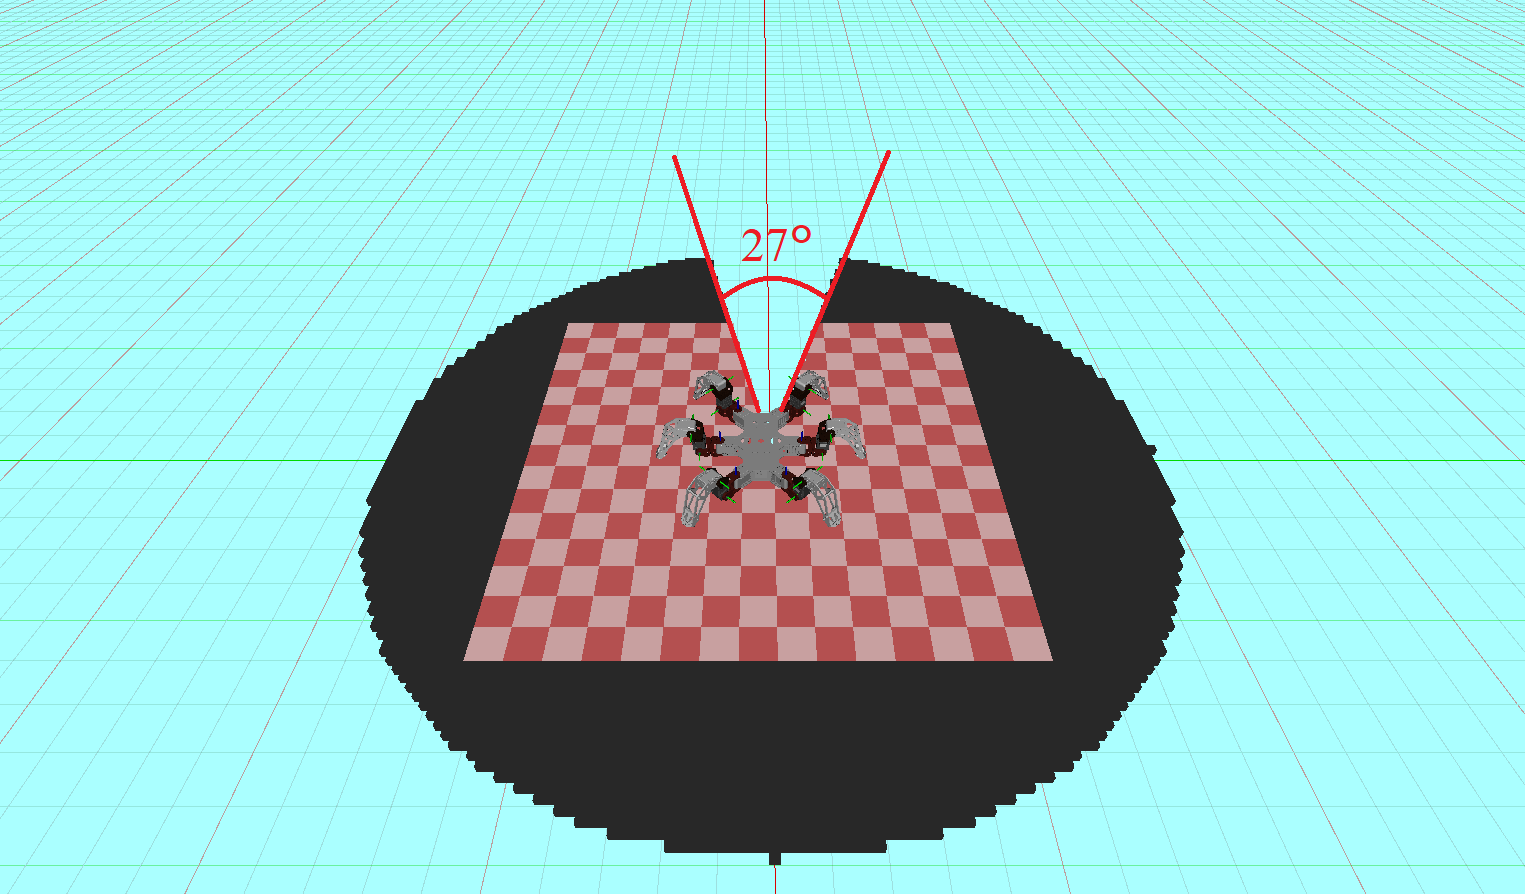
\includegraphics[width=1.0\linewidth,trim={30 30 30 30}, clip]{figure/chapter4/fissured.png}
      \text{(b) fissured terrain}
      \end{center}  
    \end{minipage}
    \\
    & \\  % 1行空ける
    \begin{minipage}[t]{0.45\hsize}
      \centering
      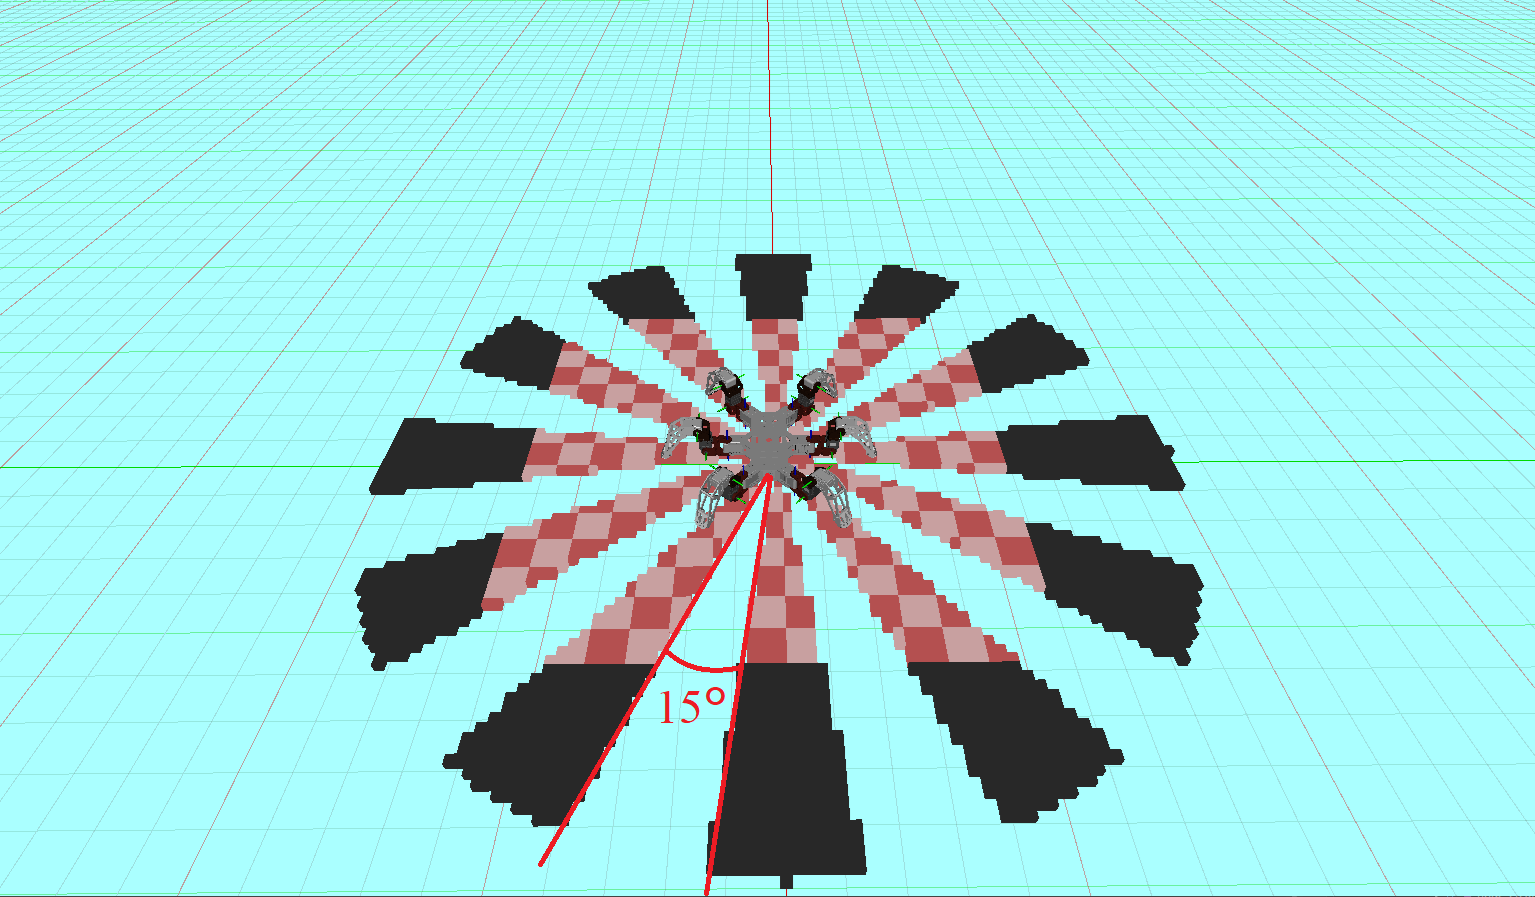
\includegraphics[width=1.0\linewidth,trim={30 30 30 30}, clip]{figure/chapter4/ditch.png}
      \centering
      \text{(c) ditched terrain}
    \end{minipage} 
    &    
    \\
  \end{tabular}
  \caption{Simulation Terrain}
  \label{fig:ch5_simu_terrain_turn} % chktex 24
\end{figure}

\begin{figure}[htbp]
  \centering
  \begin{tabular}{cc}
    \begin{minipage}[t]{0.45\hsize}
      \begin{center}
      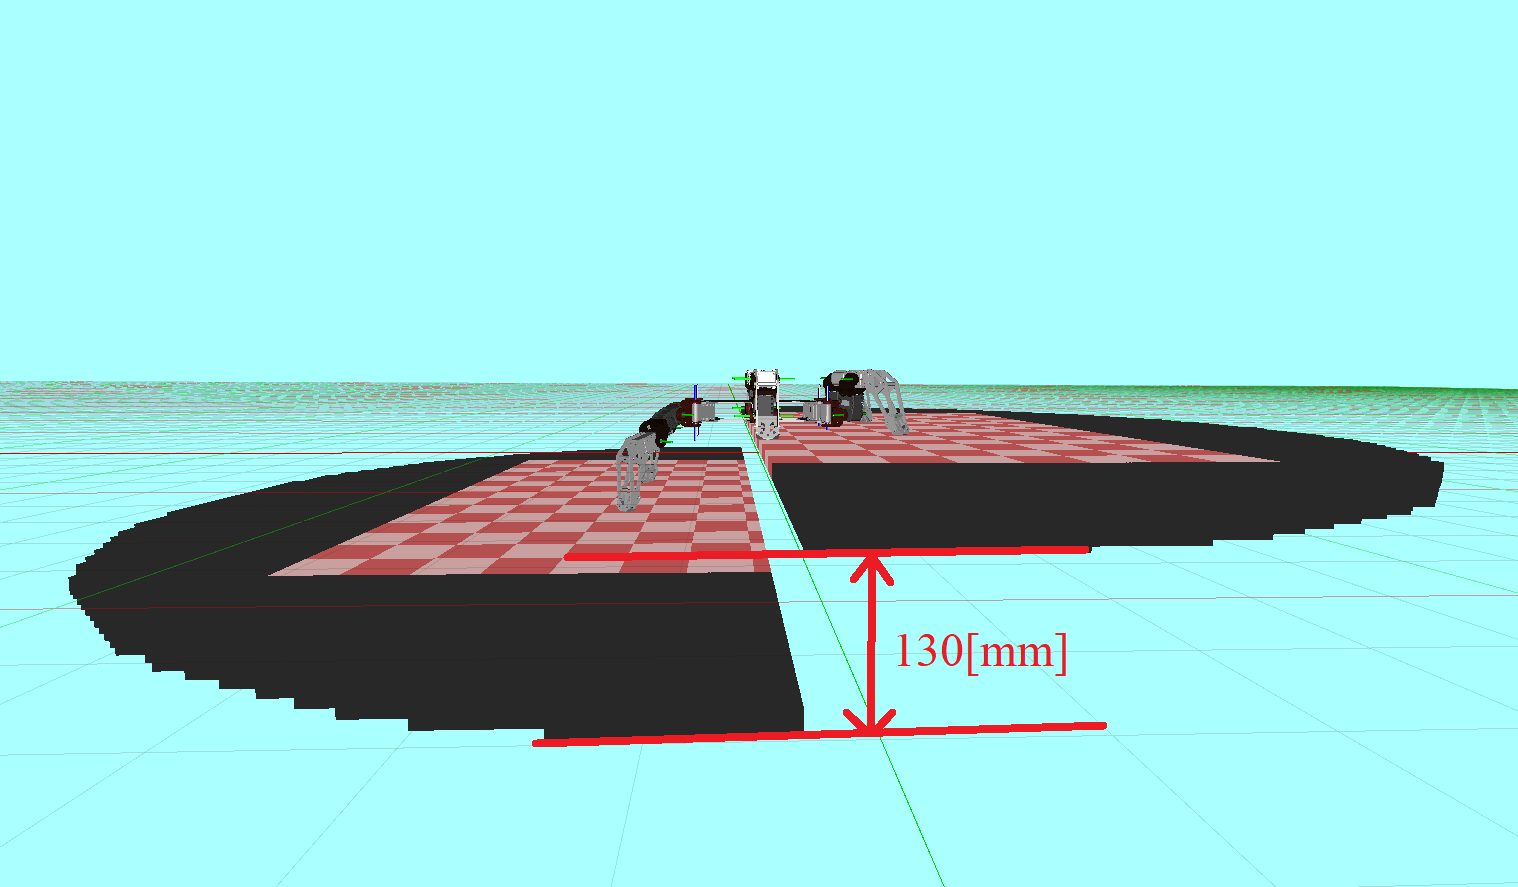
\includegraphics[width=1.0\linewidth,trim={30 30 30 30}, clip]{figure/chapter4/circle_step.png}
      \text{(a) step terrain (130mm)}
      \end{center}
    \end{minipage} 
    &
    \begin{minipage}[t]{0.45\hsize}
      \begin{center}
      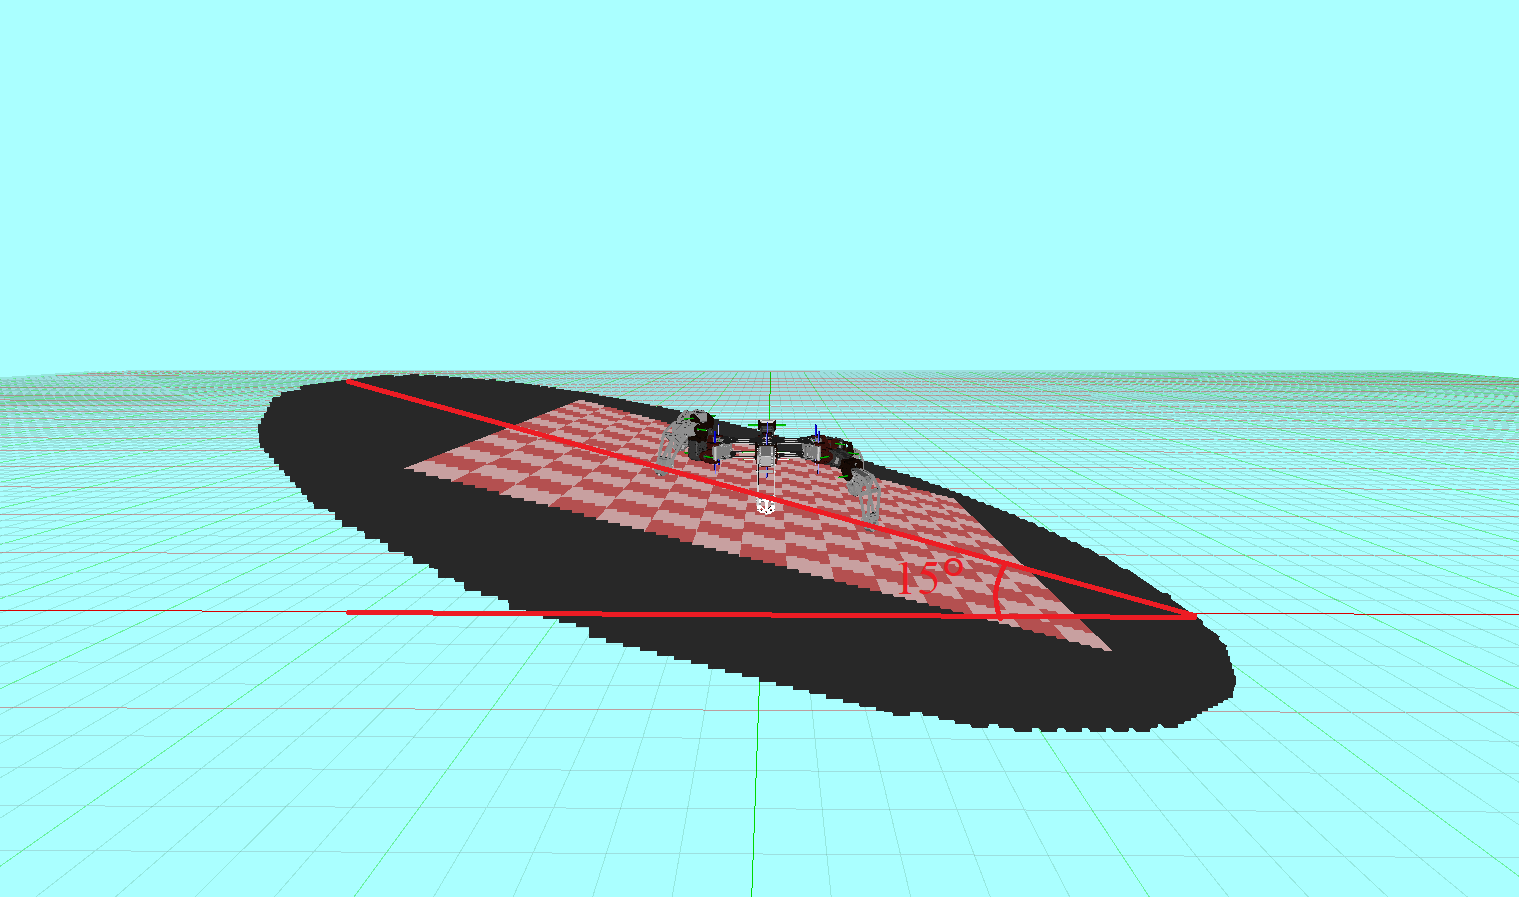
\includegraphics[width=1.0\linewidth,trim={30 30 30 30}, clip]{figure/chapter4/circle_slope.png}
      \text{(b) slope terrain ($15^{\circ}$)}
      \end{center}  
    \end{minipage}
    \\
  \end{tabular}
  \caption{Additional Terrain}
  \label{fig:ch5_simu_terrain_turn2} % chktex 24
\end{figure}

\subsubsection{シミュレーションの手順}
シミュレーションは次に示す手順で行った.
なお,旋回方向は反時計回りでシミュレーションを行った.
\begin{enumerate}
  \item ロボットの胴体を地形から30mm離れるようにロボットを配置し,脚先は地形に接触している状態となるようにする.
  \item 旋回動作を行い,胴体が重力方向を軸として360度旋回するまでの歩容パターンを生成する.
  \item 歩容パターン生成に失敗することなく,また脚軌道生成に失敗することなく,360度旋回することができた場合を成功とする.
  \item 地形を変更し,(1)から(3)を繰り返す.各地形において旋回動作が成功するかを確認する.
\end{enumerate}

\subsection{シミュレーション実験の結果}
シミュレーションの結果を\tableref{tab:ch5_simu_result_turn},\tableref{tab:ch5_simu_result_turn}に示す.
表では,各地形において旋回動作が成功した場合には「$\bigcirc$」,失敗した場合には「$\times$」と記した.
結果より,すべての地形において旋回動作が成功したとわかる.

また,\figref{fig:ch5_result_turn1},\figref{fig:ch5_result_turn2}に旋回動作を行った際の脚先座標を示す.
\figref{fig:ch5_simu_res_1}と同様に,横軸をx軸,縦軸をz軸としており,単位はmmである.
\figref{fig:ch5_range_revaluation}の$50 < x < 250$, $−200 < z < 0$の範囲を拡大したものであり,
脚先座標は支持脚時を青い丸点,遊脚時を赤い丸点,脚軌道生成に失敗した際の脚軌道の中継点を水色の$\times$で示している.
この図より,脚軌道が可動範囲外を通ることはないことがわかる.
\\

\begin{table}[htbp]
  \centering
  \caption{Simulation Result(Counter Clockwise)}
  \label{tab:ch5_simu_result_turn}  % chktex 24
  \begin{tabular}{|c|c|c|c|} \hline  % chktex 44
    & 平面 & 亀裂のある地形 & 溝がある地形 \\ \hline  % chktex 44
    変化なし & $\bigcirc$ & $\bigcirc$ & $\bigcirc$ \\ \hline  % chktex 44
    傾斜$5^{\circ}$ & $\bigcirc$ & $\bigcirc$ & $\bigcirc$ \\ \hline  % chktex 44
    傾斜$10^{\circ}$ & $\bigcirc$ & $\bigcirc$ & $\bigcirc$ \\ \hline  % chktex 44
    傾斜$15^{\circ}$ & $\bigcirc$ & $\bigcirc$ & $\bigcirc$ \\ \hline  % chktex 44
    段差100mm & $\bigcirc$ & $\bigcirc$ & $\bigcirc$ \\ \hline  % chktex 44
    段差110mm & $\bigcirc$ & $\bigcirc$ & $\bigcirc$ \\ \hline  % chktex 44
    段差120mm & $\bigcirc$ & $\bigcirc$ & $\bigcirc$ \\ \hline  % chktex 44
    段差130mm & $\bigcirc$ & $\bigcirc$ & $\bigcirc$ \\ \hline  % chktex 44
  \end{tabular}
\end{table}


\begin{figure}[htbp]
  \centering
  \begin{tabular}{ccc}
    \begin{minipage}[t]{0.28\linewidth}
      \begin{center}
      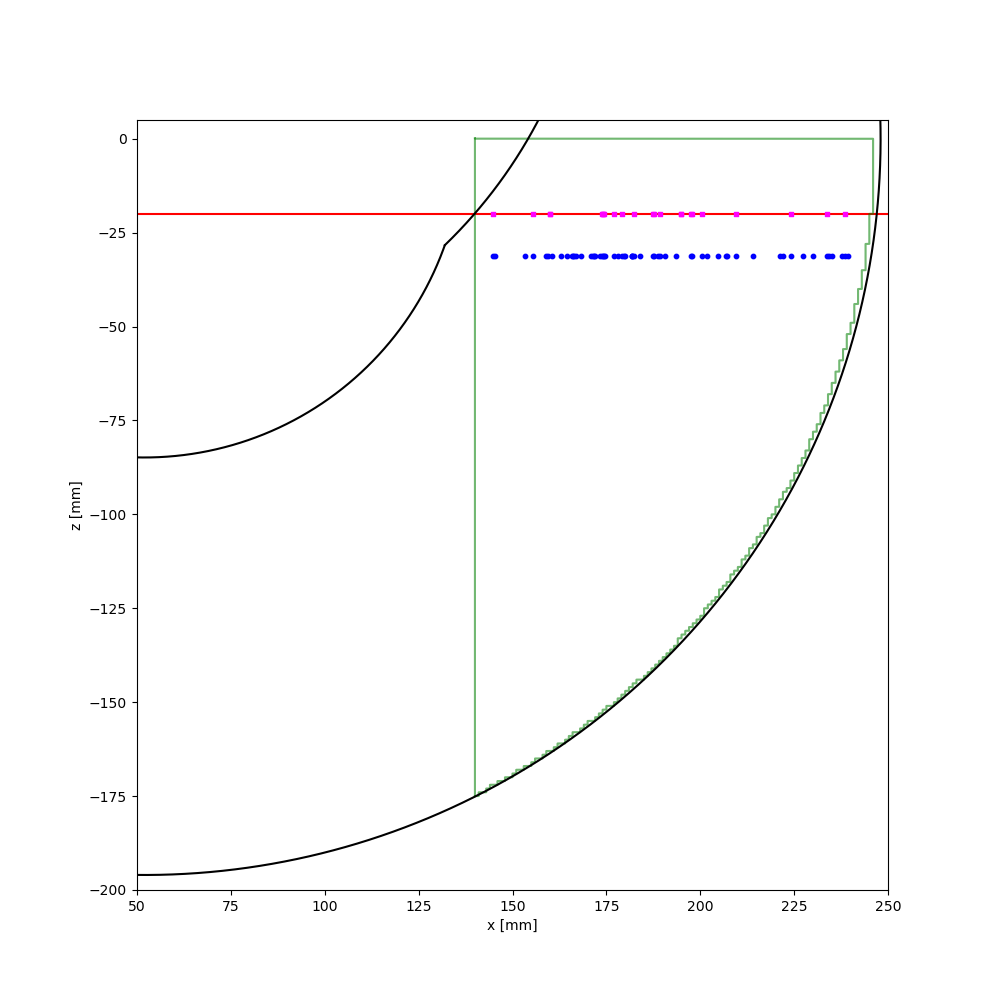
\includegraphics[width=1.0\linewidth,trim={30 30 30 30}, clip]{figure/chapter4/turn/flat_none.png}
      \text{(a) flat}
      \end{center}
    \end{minipage} 
    &
    \begin{minipage}[t]{0.28\linewidth}
      \begin{center}
      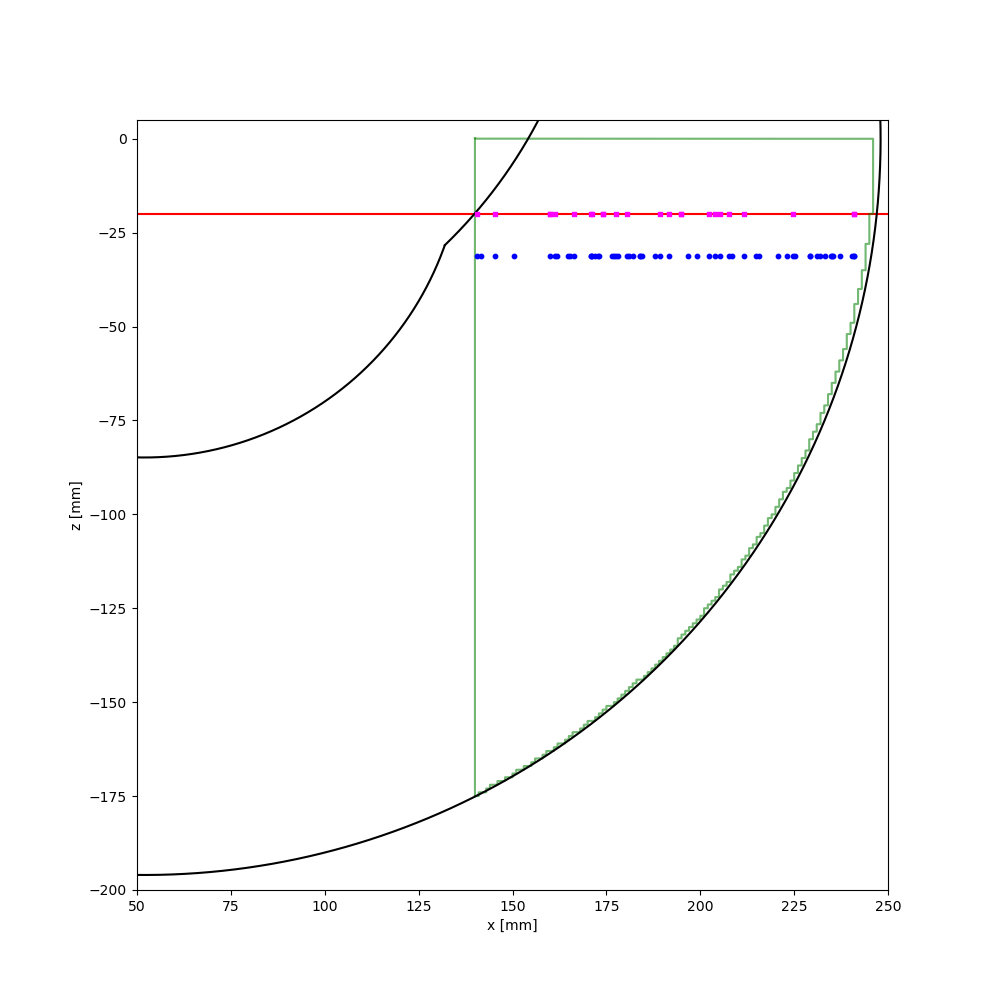
\includegraphics[width=1.0\linewidth,trim={30 30 30 30}, clip]{figure/chapter4/turn/fissured_none.png}
      \text{(b) fissured}
      \end{center}  
    \end{minipage}
    &
    \begin{minipage}[t]{0.28\linewidth}
      \begin{center}
      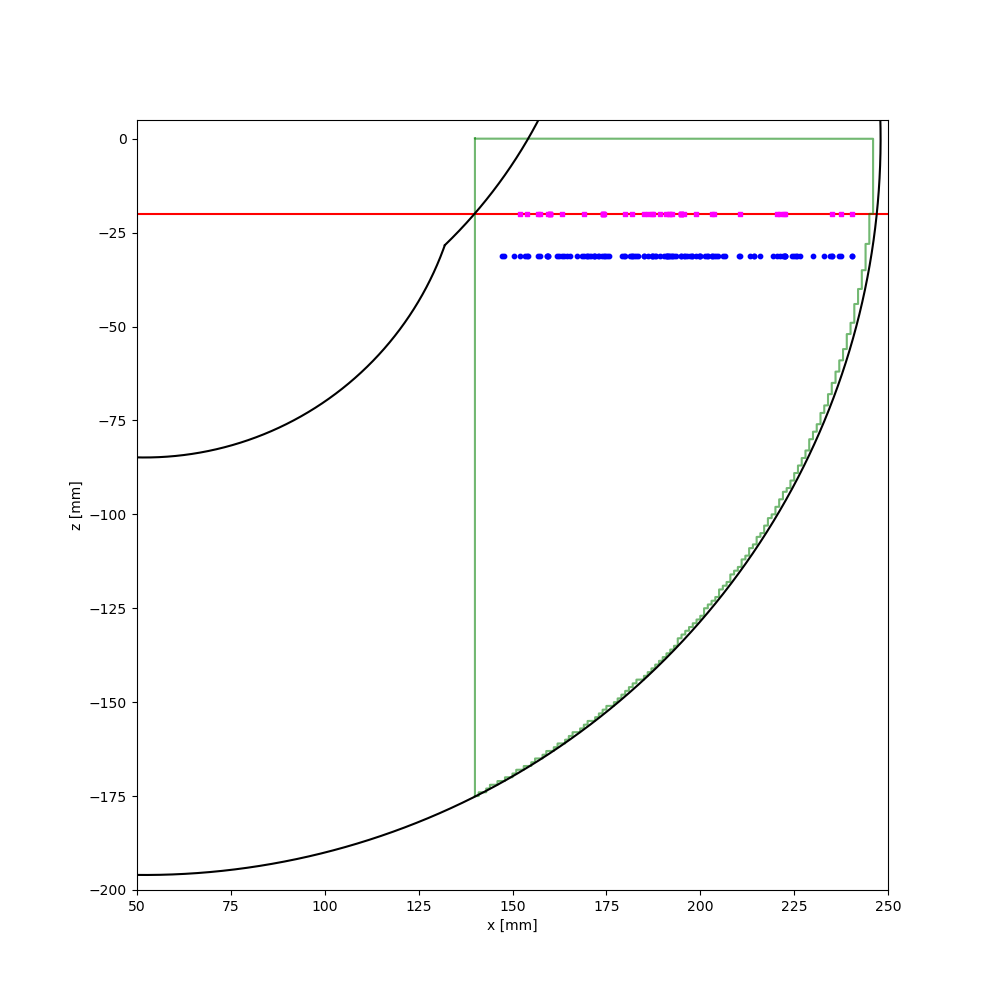
\includegraphics[width=1.0\linewidth,trim={30 30 30 30}, clip]{figure/chapter4/turn/ditch_none.png}
      \text{(c) ditched}
    \end{center}
    \end{minipage}    
    \\
    \begin{minipage}[t]{0.28\linewidth}
      \begin{center}
      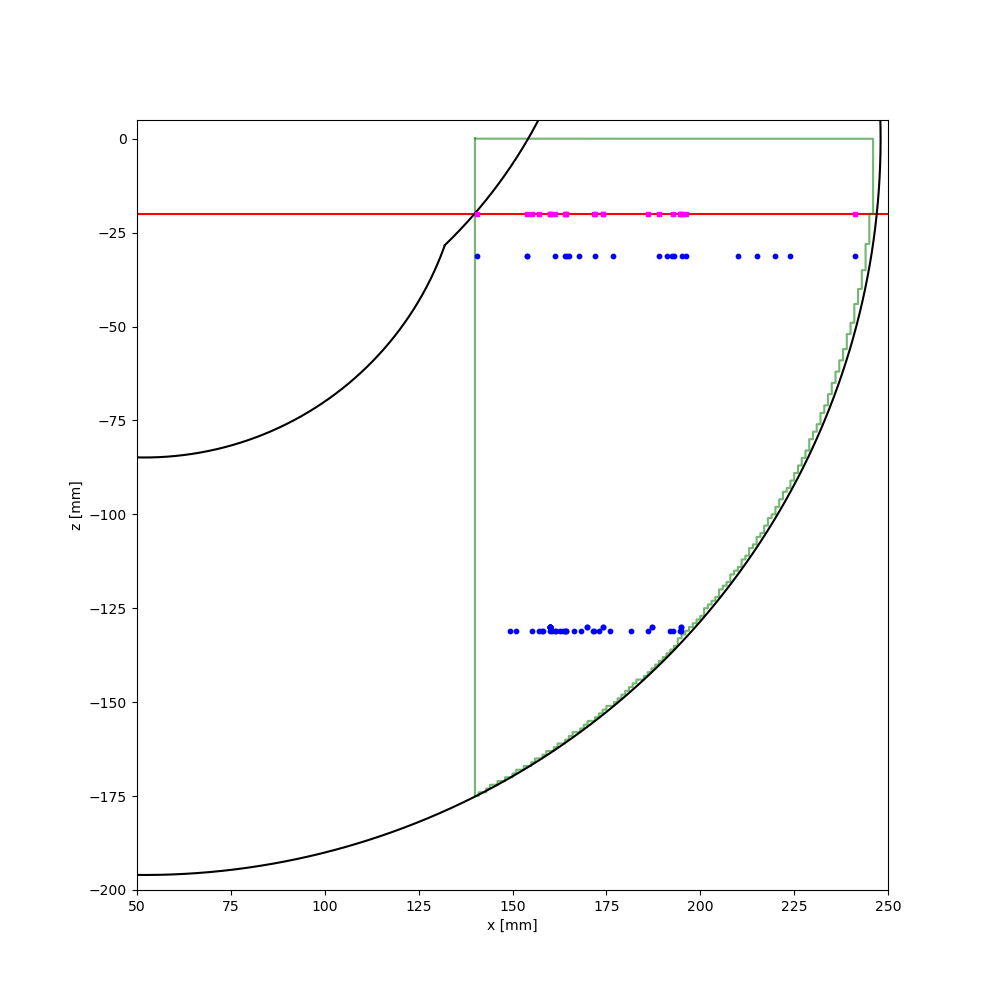
\includegraphics[width=1.0\linewidth,trim={30 30 30 30}, clip]{figure/chapter4/turn/flat_100mm.png}
      \text{(d) flat 100mm step}
      \end{center}
    \end{minipage}
    &
    \begin{minipage}[t]{0.28\linewidth}
      \begin{center}
      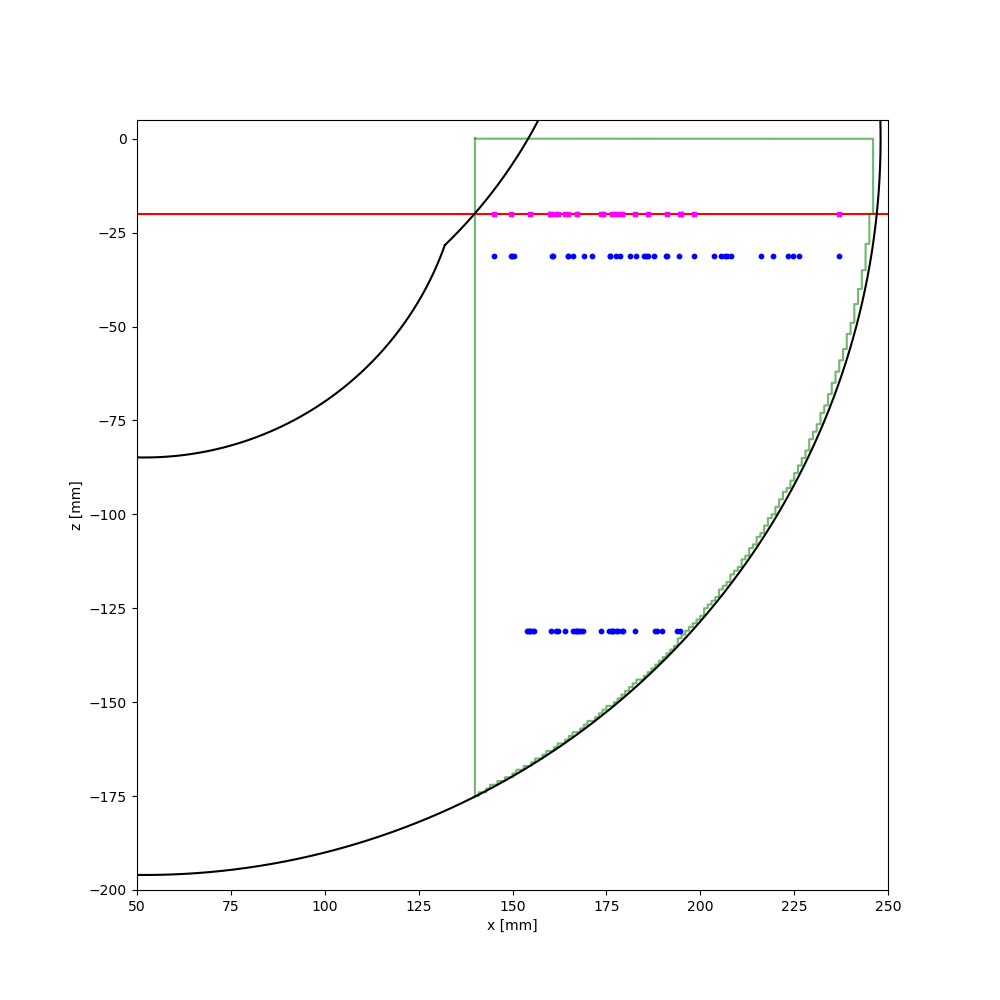
\includegraphics[width=1.0\linewidth,trim={30 30 30 30}, clip]{figure/chapter4/turn/fissured_100mm.png}
      \text{(e) fissured 100mm step}
      \end{center}
    \end{minipage}
    &
    \begin{minipage}[t]{0.28\linewidth}
      \begin{center}
      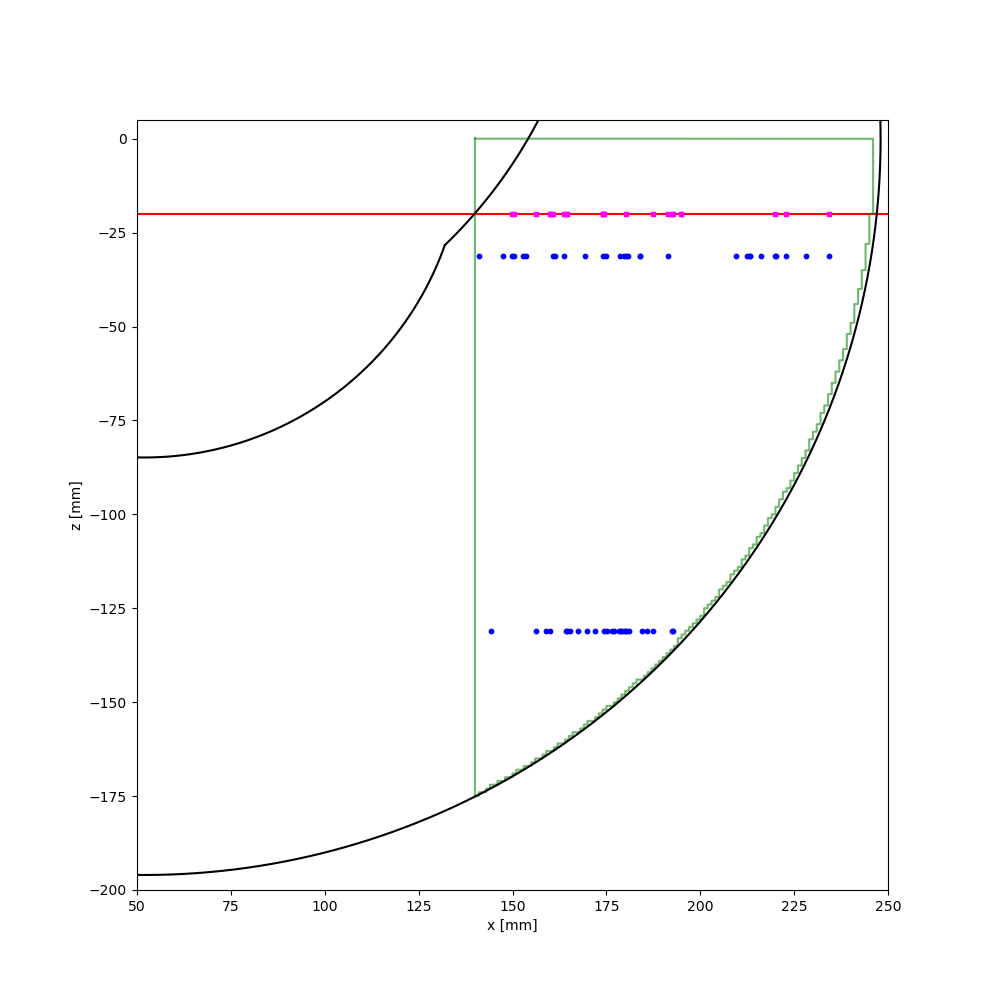
\includegraphics[width=1.0\linewidth,trim={30 30 30 30}, clip]{figure/chapter4/turn/ditch_100mm.png}
      \text{(f) ditched 100mm step}
      \end{center}
    \end{minipage}
    \\
    \begin{minipage}[t]{0.28\linewidth}
      \begin{center}
      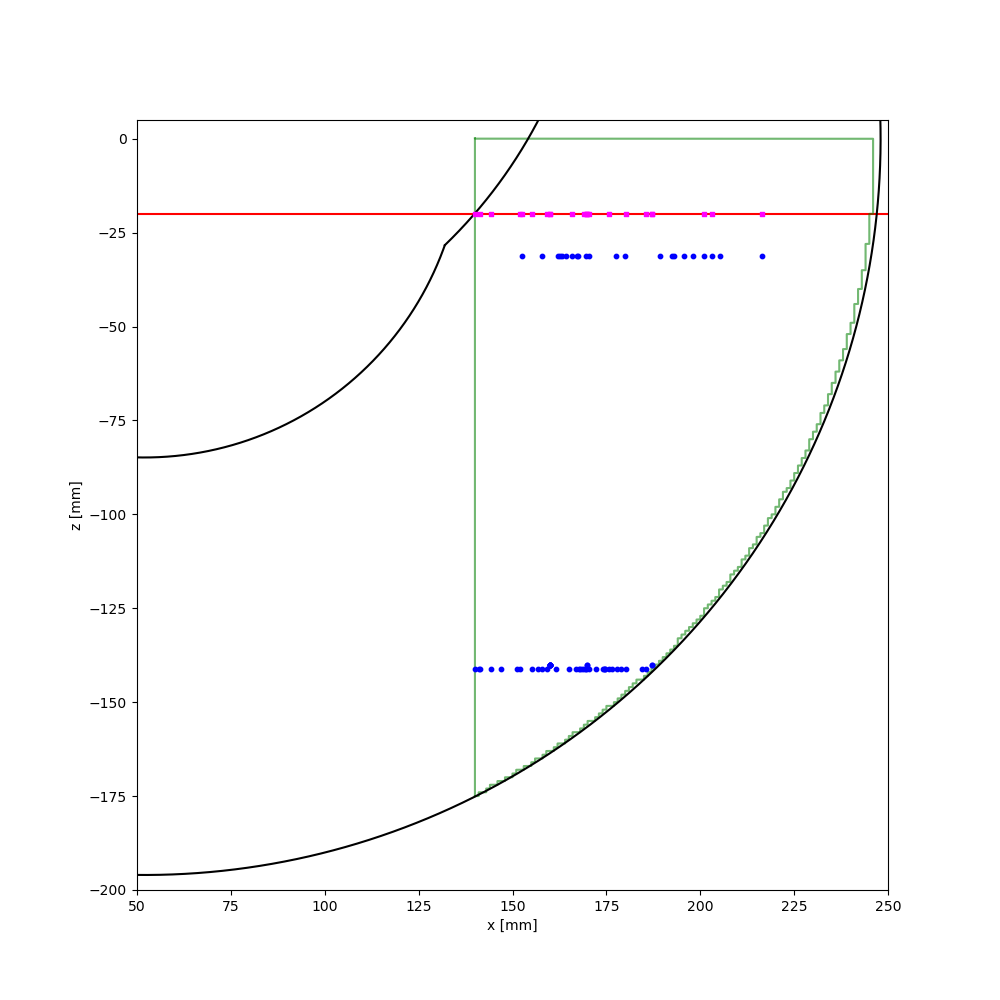
\includegraphics[width=1.0\linewidth,trim={30 30 30 30}, clip]{figure/chapter4/turn/flat_110mm.png}
      \text{(g) flat 110mm step}
      \end{center}
    \end{minipage}
    &
    \begin{minipage}[t]{0.28\linewidth}
      \begin{center}
      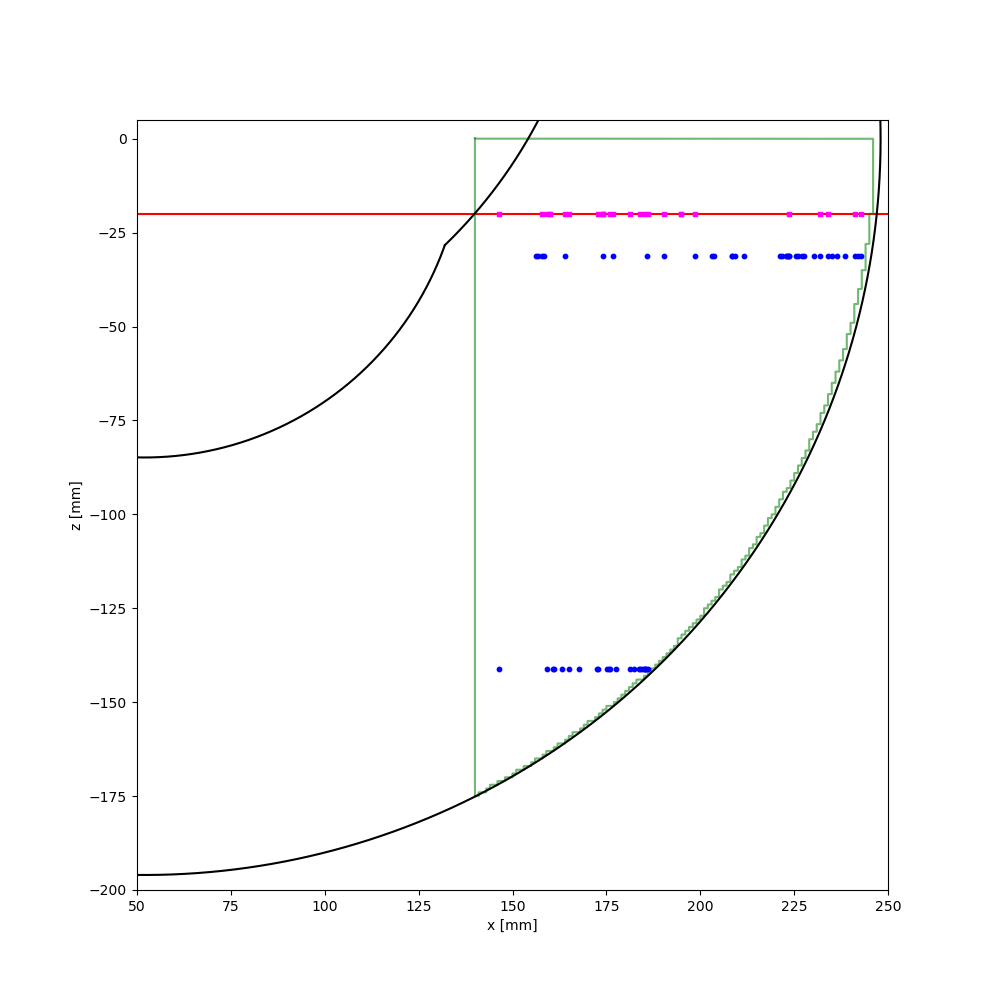
\includegraphics[width=1.0\linewidth,trim={30 30 30 30}, clip]{figure/chapter4/turn/fissured_110mm.png}
      \text{(h) fissured 110mm step}
      \end{center}
    \end{minipage}
    &
    \begin{minipage}[t]{0.28\linewidth}
      \begin{center}
      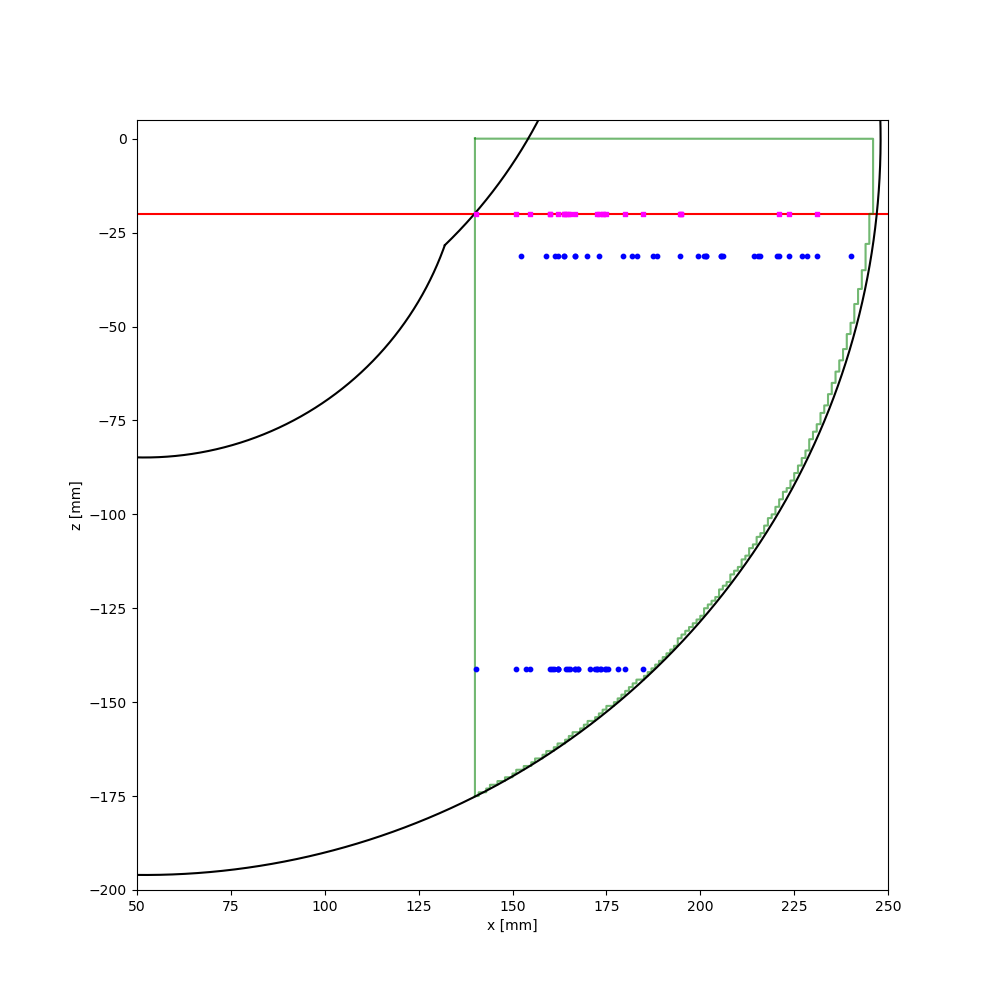
\includegraphics[width=1.0\linewidth,trim={30 30 30 30}, clip]{figure/chapter4/turn/ditch_110mm.png}
      \text{(i) ditched 110mm step}
      \end{center}
    \end{minipage}
    \\
    \begin{minipage}[t]{0.28\linewidth}
      \begin{center}
      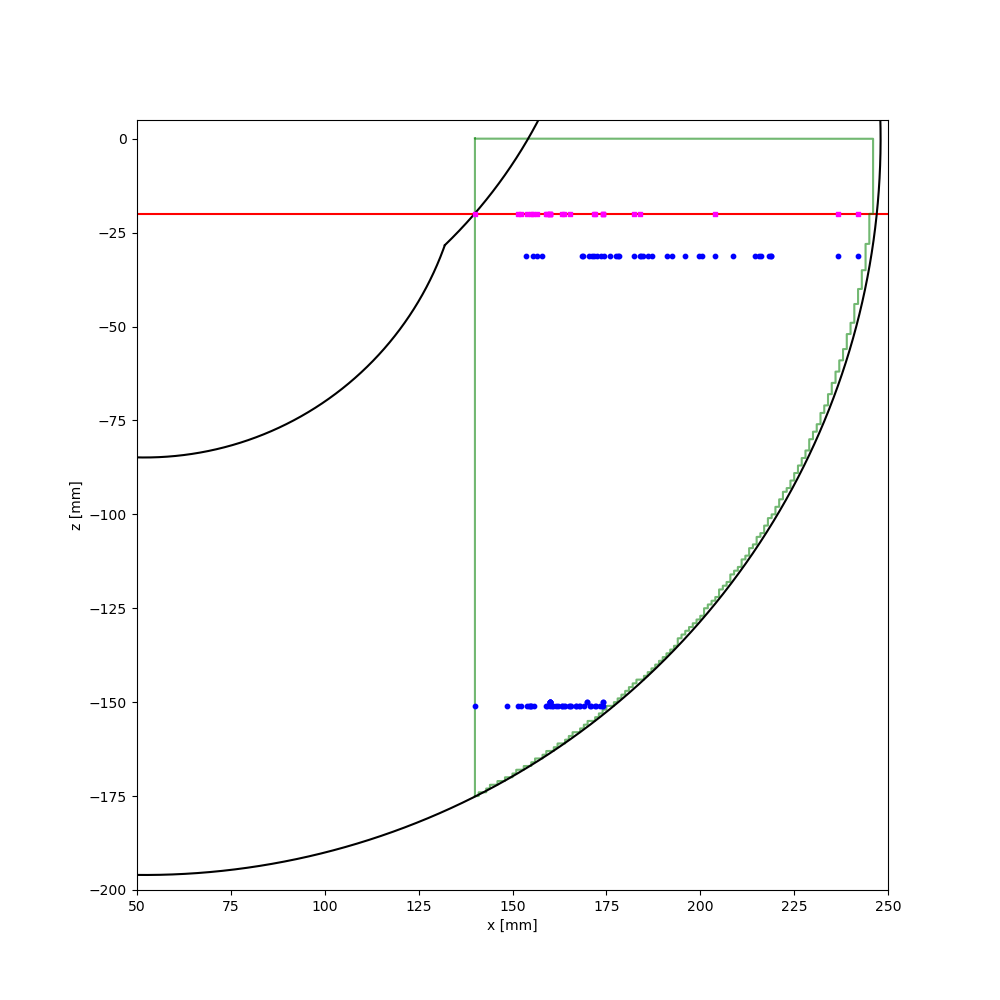
\includegraphics[width=1.0\linewidth,trim={30 30 30 30}, clip]{figure/chapter4/turn/flat_120mm.png}
      \text{(j) flat 120mm step}
      \end{center}
    \end{minipage}
    &
    \begin{minipage}[t]{0.28\linewidth}
      \begin{center}
      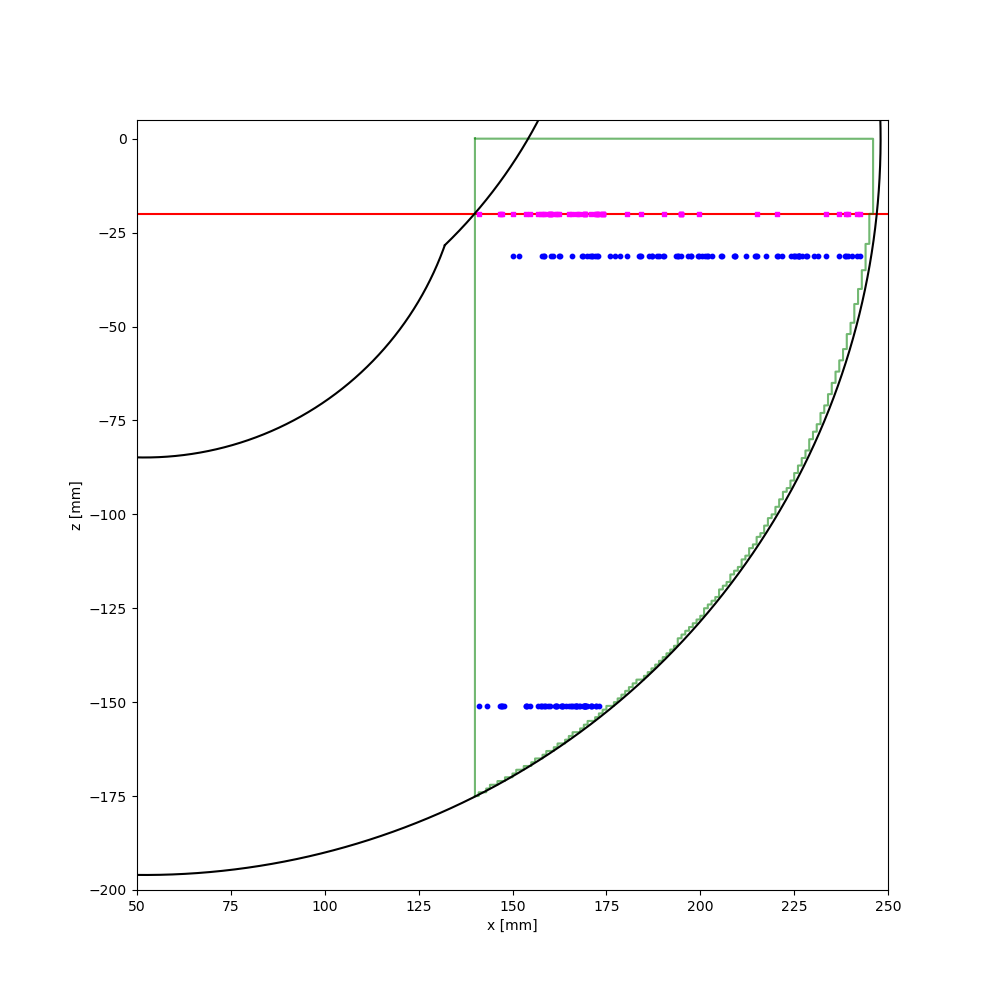
\includegraphics[width=1.0\linewidth,trim={30 30 30 30}, clip]{figure/chapter4/turn/fissured_120mm.png}
      \text{(k) fissured 120mm step}
      \end{center}
    \end{minipage}
    &
    \begin{minipage}[t]{0.28\linewidth}
      \begin{center}
      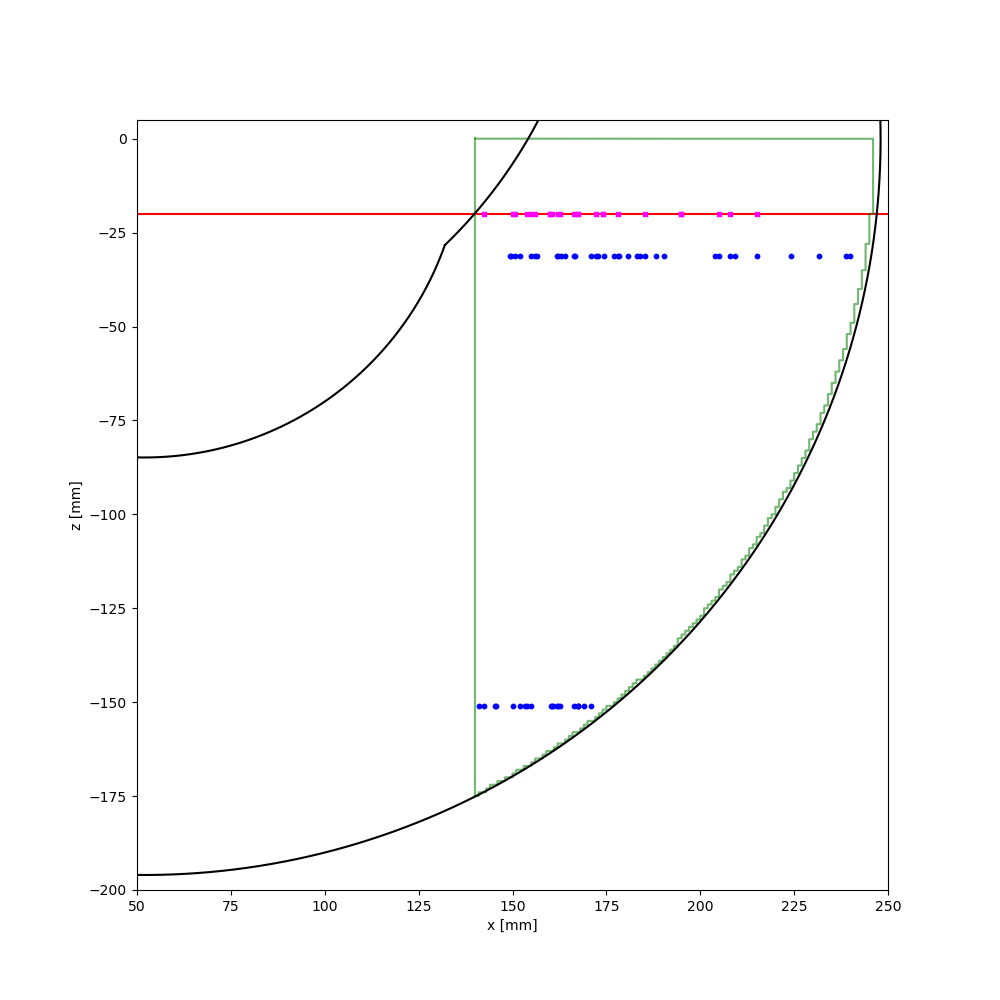
\includegraphics[width=1.0\linewidth,trim={30 30 30 30}, clip]{figure/chapter4/turn/ditch_120mm.png}
      \text{(l) ditched 120mm step}
      \end{center}
    \end{minipage}
    \\    
  \end{tabular}
  \caption{Leg Ground Points for Each Terrain (Turn Move)}
  \label{fig:ch5_result_turn1} % chktex 24
\end{figure}

\begin{figure}[htbp]
  \centering
  \begin{tabular}{ccc}
    \begin{minipage}[t]{0.28\linewidth}
      \begin{center}
      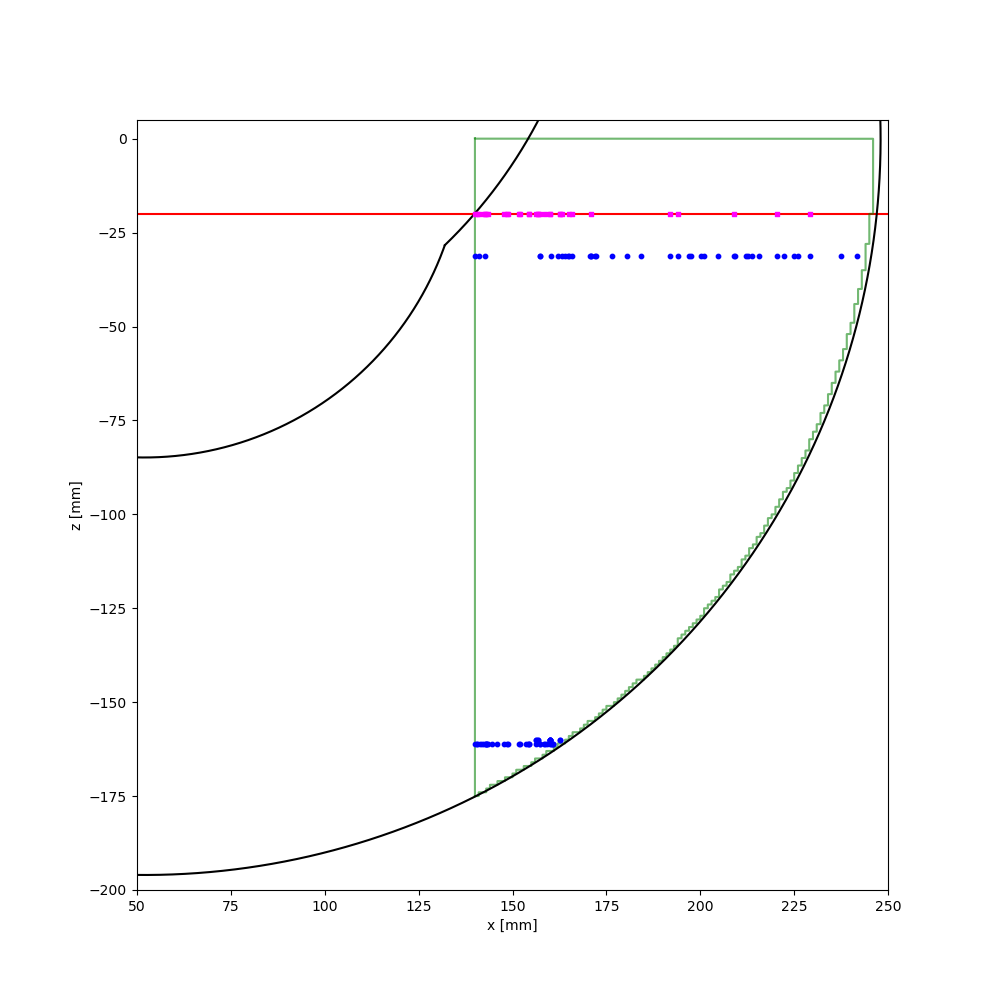
\includegraphics[width=1.0\linewidth,trim={30 30 30 30}, clip]{figure/chapter4/turn/flat_130mm.png}
      \text{(m) flat 130mm step}
      \end{center}
    \end{minipage}
    &
    \begin{minipage}[t]{0.28\linewidth}
      \begin{center}
      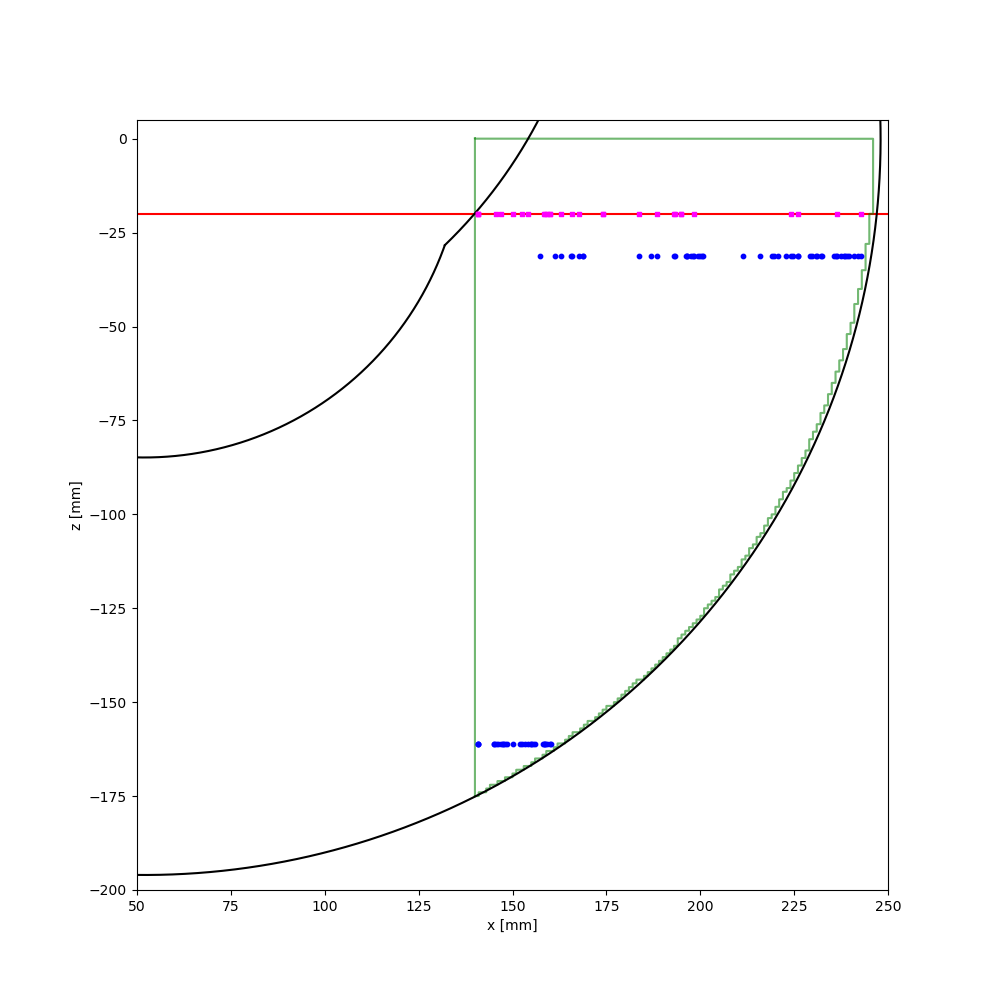
\includegraphics[width=1.0\linewidth,trim={30 30 30 30}, clip]{figure/chapter4/turn/fissured_130mm.png}
      \text{(n) fissured 130mm step}
      \end{center}
    \end{minipage}
    &
    \begin{minipage}[t]{0.28\linewidth}
      \begin{center}
      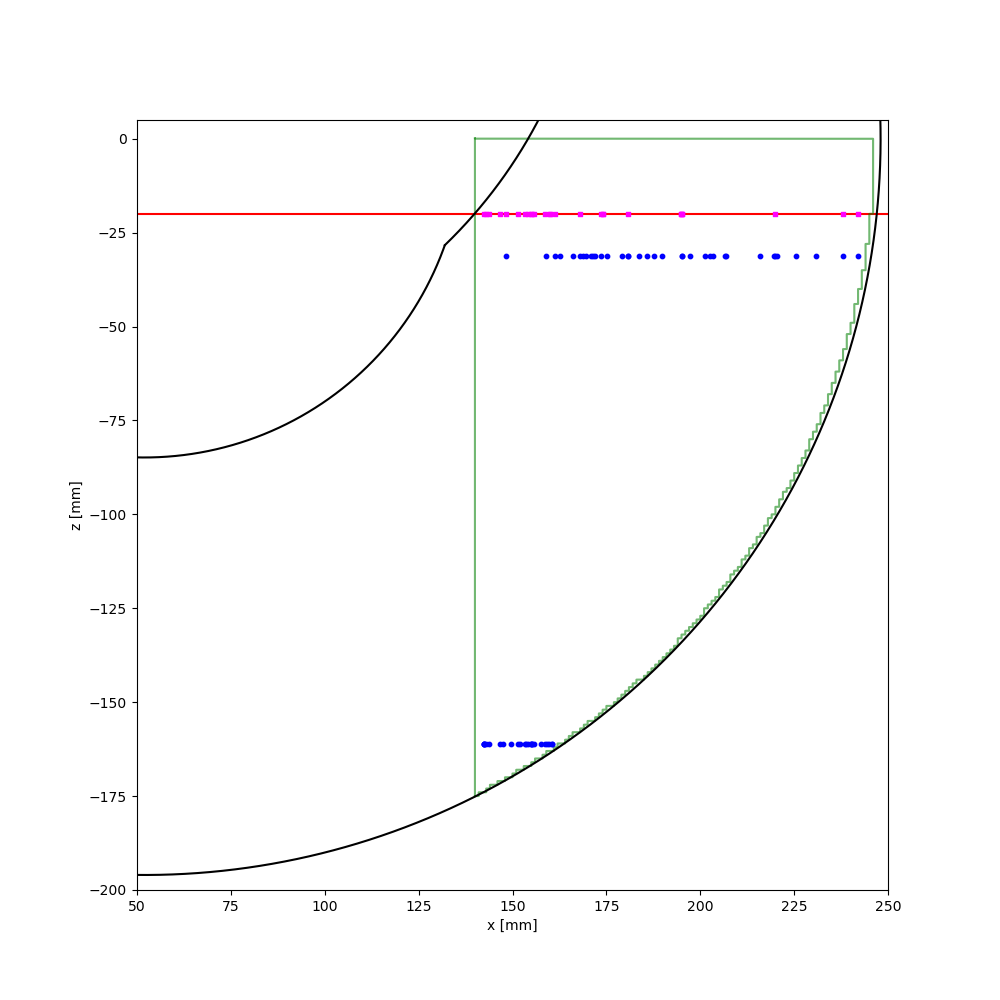
\includegraphics[width=1.0\linewidth,trim={30 30 30 30}, clip]{figure/chapter4/turn/ditch_130mm.png}
      \text{(o) ditched 130mm step}
    \end{center}
    \end{minipage}
    \\
    \begin{minipage}[t]{0.28\linewidth}
      \begin{center}
      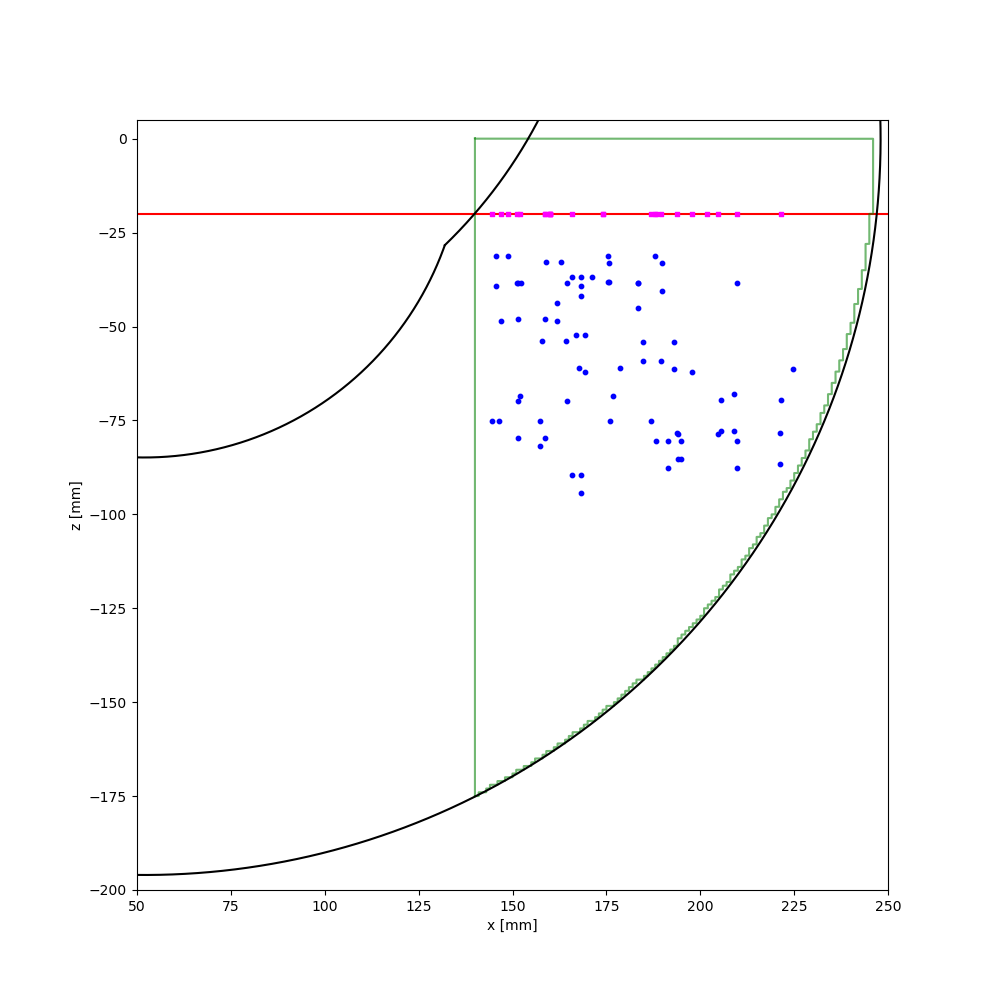
\includegraphics[width=1.0\linewidth,trim={30 30 30 30}, clip]{figure/chapter4/turn/flat_5deg.png}
      \text{(p) flat $5^{\circ}$ slope}
      \end{center}
    \end{minipage}
    &
    \begin{minipage}[t]{0.28\linewidth}
      \begin{center}
      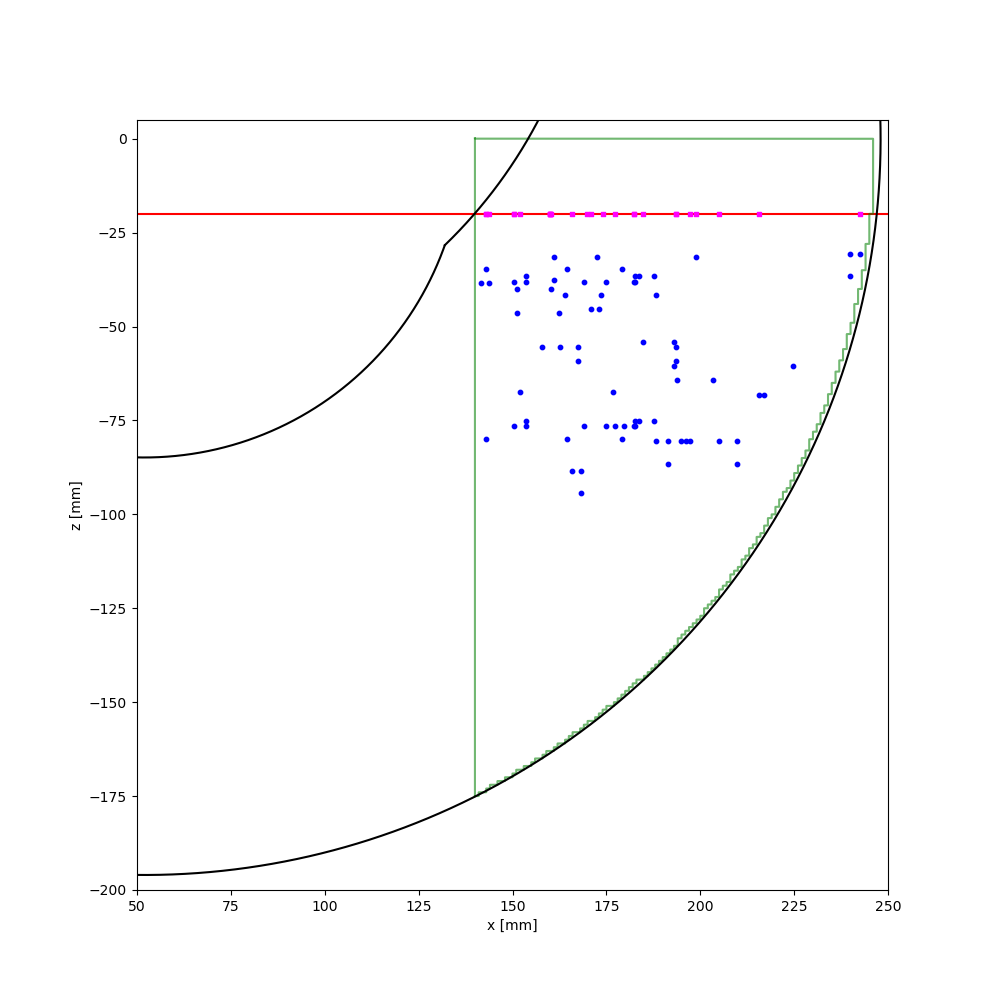
\includegraphics[width=1.0\linewidth,trim={30 30 30 30}, clip]{figure/chapter4/turn/fissured_5deg.png}
      \text{(q) fissured $5^{\circ}$ slope}
      \end{center}
    \end{minipage}
    &
    \begin{minipage}[t]{0.28\linewidth}
      \begin{center}
      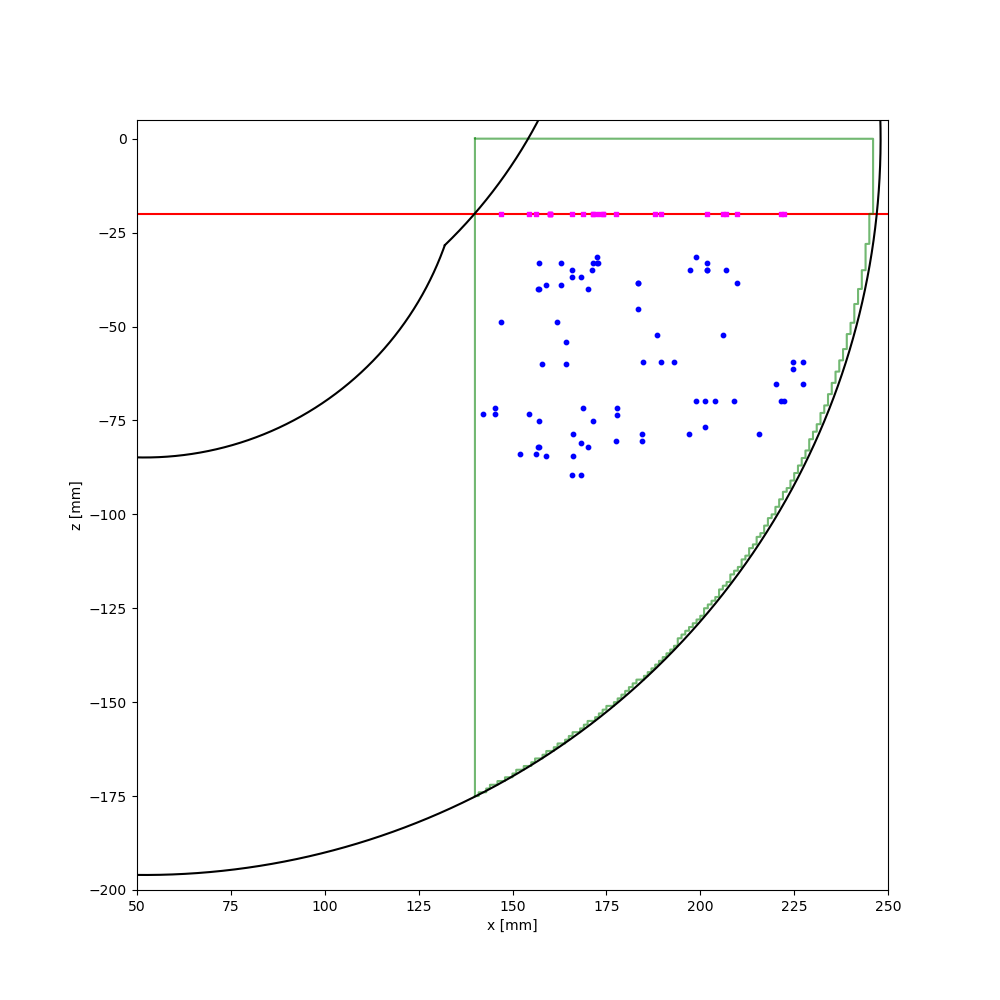
\includegraphics[width=1.0\linewidth,trim={30 30 30 30}, clip]{figure/chapter4/turn/ditch_5deg.png}
      \text{(r) ditched $5^{\circ}$ slope}
      \end{center}
    \end{minipage}
    \\
    \begin{minipage}[t]{0.28\linewidth}
      \begin{center}
      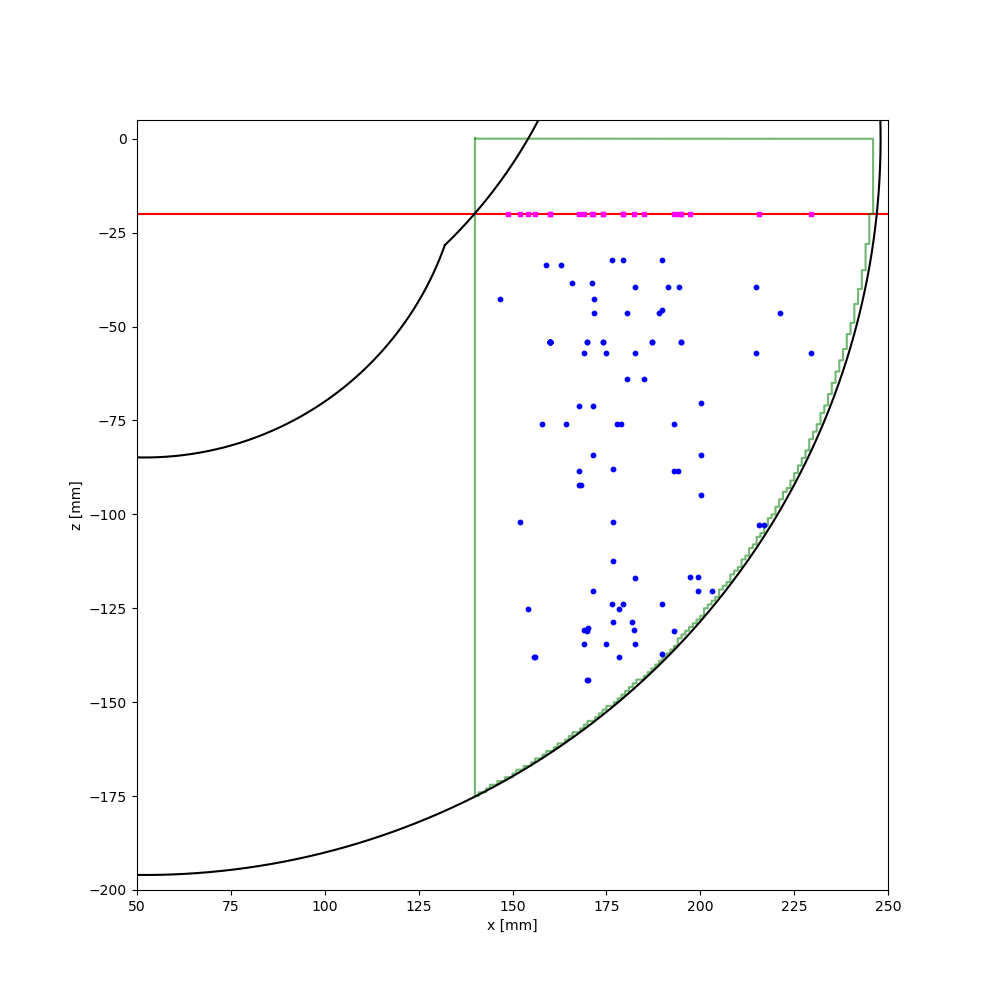
\includegraphics[width=1.0\linewidth,trim={30 30 30 30}, clip]{figure/chapter4/turn/flat_10deg.png}
      \text{(s) flat $10^{\circ}$ slope}
      \end{center}
    \end{minipage}
    &
    \begin{minipage}[t]{0.28\linewidth}
      \begin{center}
      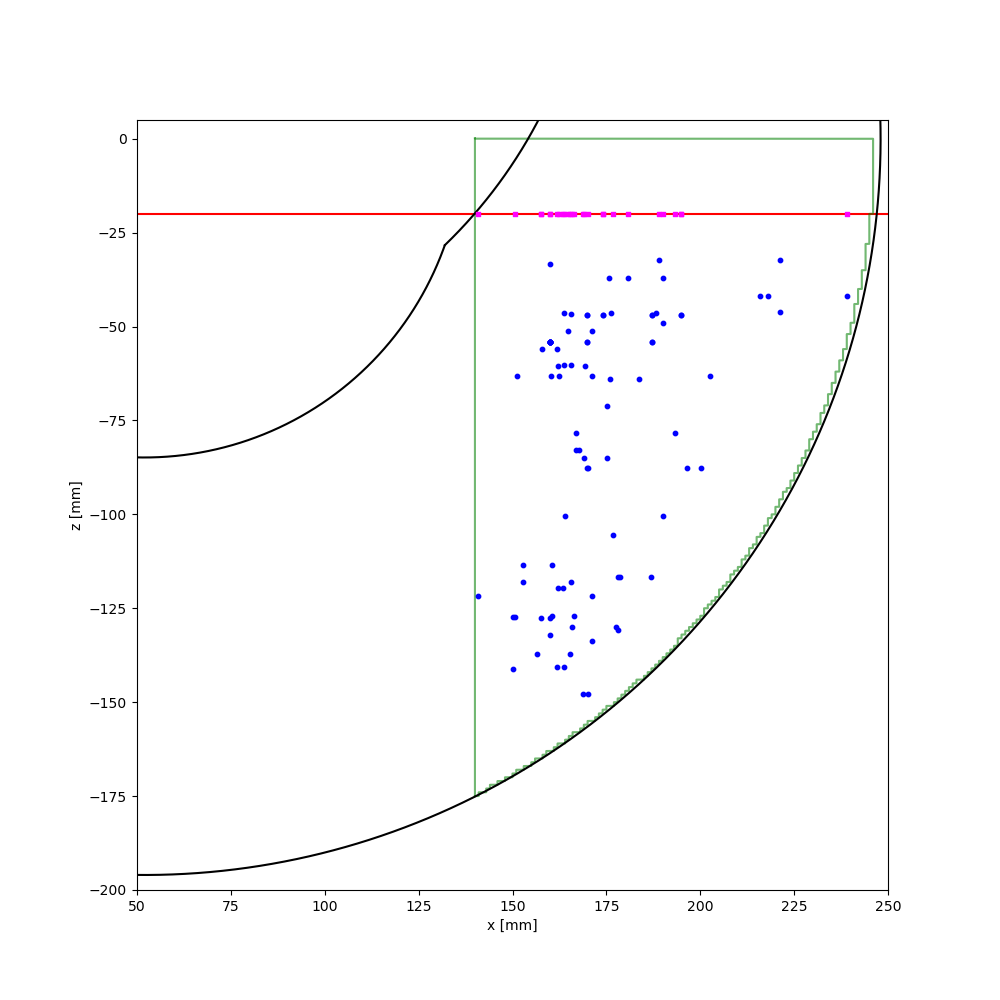
\includegraphics[width=1.0\linewidth,trim={30 30 30 30}, clip]{figure/chapter4/turn/fissured_10deg.png}
      \text{(t) fissured $10^{\circ}$ slope}
      \end{center}
    \end{minipage}
    &
    \begin{minipage}[t]{0.28\linewidth}
      \begin{center}
      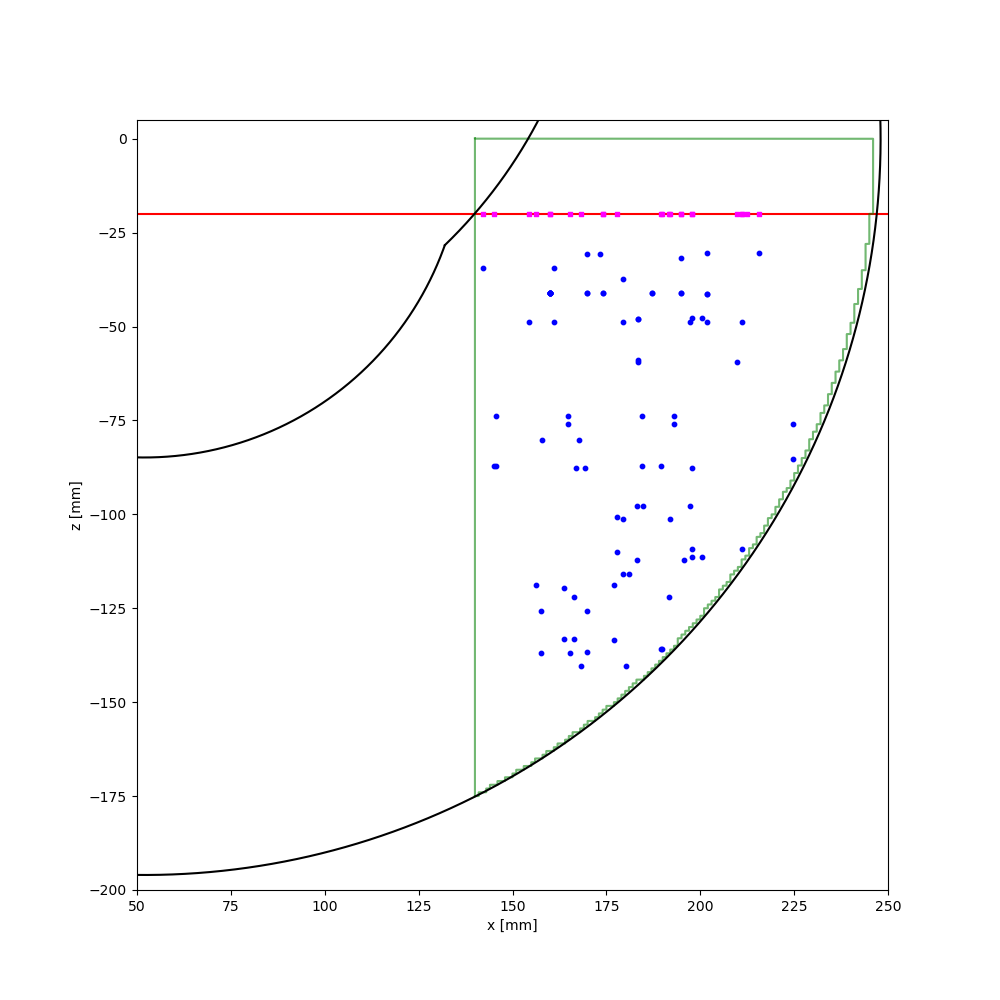
\includegraphics[width=1.0\linewidth,trim={30 30 30 30}, clip]{figure/chapter4/turn/ditch_10deg.png}
      \text{(u) ditched $10^{\circ}$ slope}
      \end{center}
    \end{minipage}
    \\
    \begin{minipage}[t]{0.28\linewidth}
      \begin{center}
      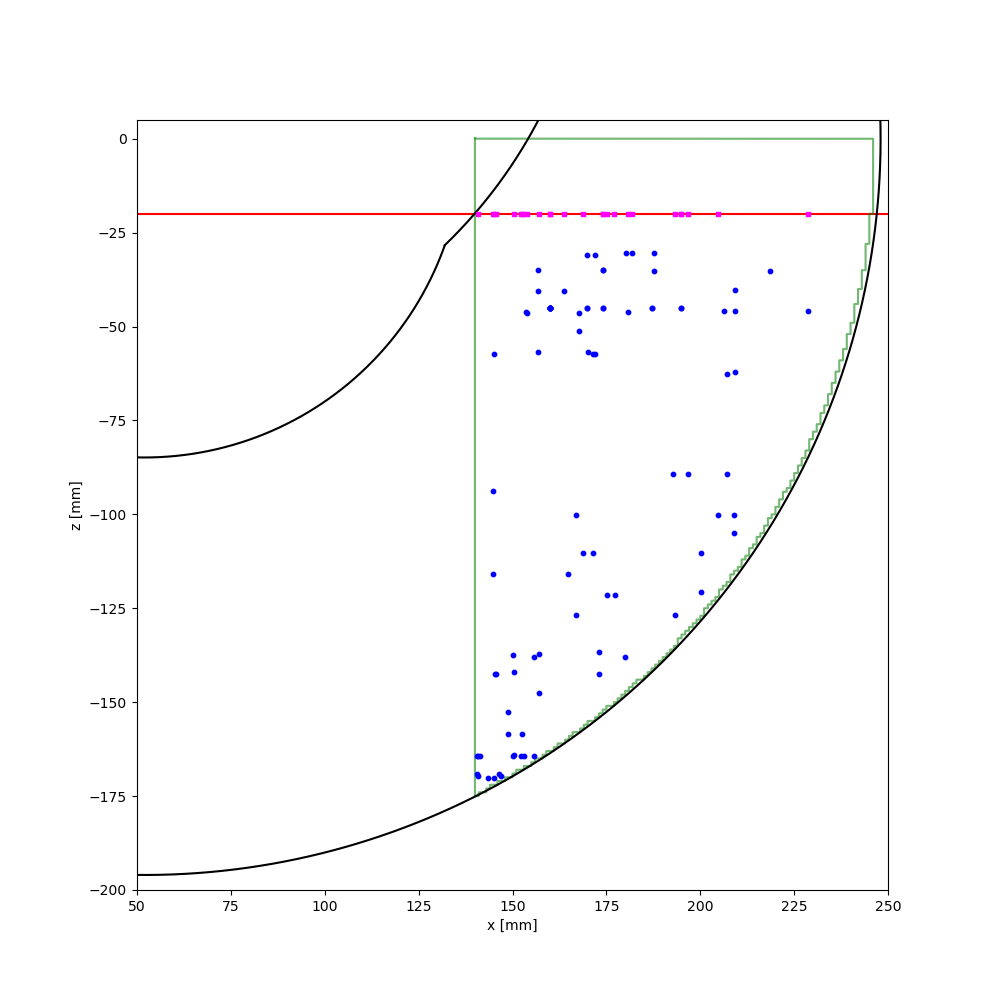
\includegraphics[width=1.0\linewidth,trim={30 30 30 30}, clip]{figure/chapter4/turn/flat_15deg.png}
      \text{(v) flat $15^{\circ}$ slope}
      \end{center}
    \end{minipage}
    &
    \begin{minipage}[t]{0.28\linewidth}
      \begin{center}
      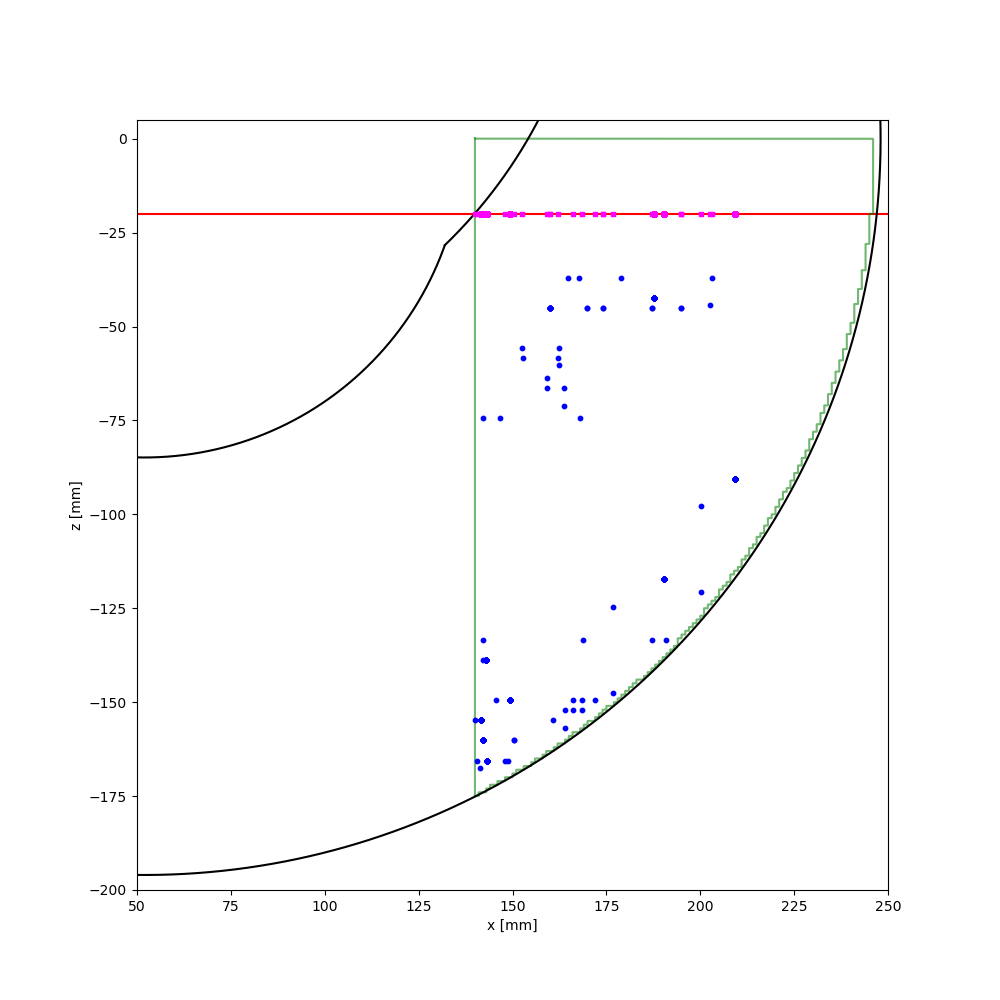
\includegraphics[width=1.0\linewidth,trim={30 30 30 30}, clip]{figure/chapter4/turn/fissured_15deg.png}
      \text{(w) fissured $15^{\circ}$ slope}
      \end{center}
    \end{minipage}
    &
    \begin{minipage}[t]{0.28\linewidth}
      \begin{center}
      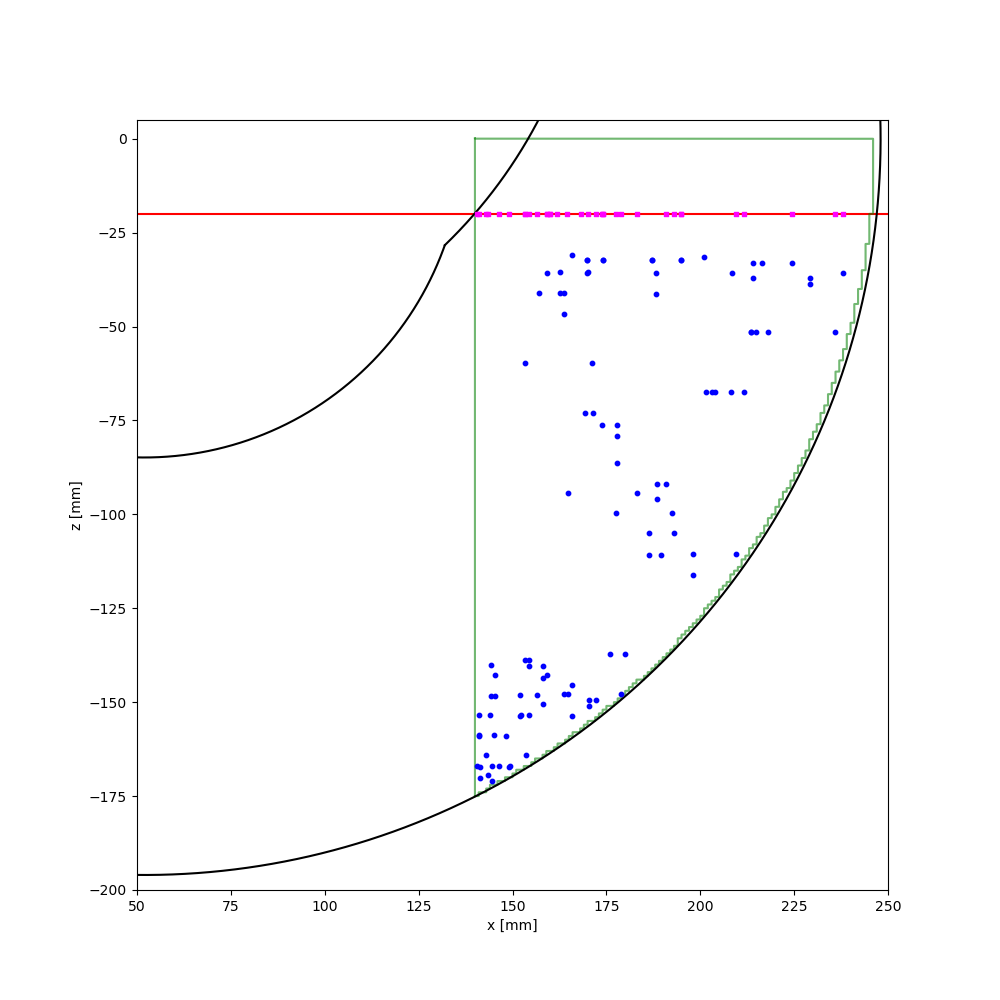
\includegraphics[width=1.0\linewidth,trim={30 30 30 30}, clip]{figure/chapter4/turn/ditch_15deg.png}
      \text{(x) ditched $15^{\circ}$ slope}
      \end{center}
    \end{minipage}
    \\
  \end{tabular}
  \caption{Leg Ground Points for Each Terrain (Turn Move)}
  \label{fig:ch5_result_turn2} % chktex 24
\end{figure}

\subsection{考察}
傾斜や段差がない場合,すべての地形で旋回動作を行うことができたため,
最小半径を140mmに設定したとしても,
先行研究で歩行することができた地形を歩行することができなくなってしまうことはないことがわかった.
また,3次元空間においてもすべての地形で旋回動作が成功したことから,
3次元空間でも旋回動作が可能であるとわかった.

これらの地形で旋回動作を行うことができた理由として,
各地形を旋回する上で必要な高さまで脚先を下げることができたためと考えられる.


結論として,最小半径を140mmとした場合でも,旋回動作を行うことができることを確認できた.